%---------------DOCUMENT SETTINGS------------------------------------
%\documentclass[headheight=30pt]{scrartcl}
\documentclass{article}

\usepackage[utf8]{inputenc} % utf8x durch utf8 ersetzt wegen biblatex
\usepackage[T1]{fontenc}
\usepackage{amsmath,amssymb,amstext,amsfonts}
\usepackage[english]{babel}
\usepackage{csquotes}
\usepackage{pdfpages} %zum importieren des Deckblattes
\usepackage{geometry}
\usepackage[headsepline]{scrlayer-scrpage}
\usepackage{lastpage}
\usepackage[style=numeric]{biblatex} %Literaturverwaltung
\usepackage{tabularx} %für die Legende im Gruundlagen Oszi Bild
\usepackage{float}
\usepackage{textcomp}
\usepackage{gensymb}
\usepackage{physics}
\usepackage{stmaryrd}
\usepackage{graphicx}
\usepackage[export]{adjustbox}
\usepackage{a4wide}
\usepackage[separate-uncertainty=true]{siunitx}
\usepackage[hidelinks]{hyperref}
\usepackage{multicol}
\usepackage{makecell}
\usepackage{wrapfig}
\usepackage[justification=centering]{caption}
\usepackage{textcomp}
\usepackage{subcaption}

\DeclareSIUnit\molecule{molecule}

\geometry{      %holt mehr aus einer A4 Seite raus
    a4paper,
    total={170mm,257mm},
    left=20mm,
    top=25mm,
   }
\graphicspath{ {./graphics/} }  %pfad für bilder
\hypersetup{colorlinks=false}
\addbibresource{literatur.bib} %Literatur-Resourcen
%\setlength{\headheight}{0.0pt} % macht zwar headheight warnings aber dafür nutz latex die seitengröße besser aus.
\pagestyle{scrheadings}
\newcommand{\duofigcom}[6]{
    \begin{figure}[H]
        \centering
        \begin{subfigure}{0.9\textwidth}
            \includegraphics[width=\textwidth]{#1}
            \caption{}
            \label{#2}
        \end{subfigure}
        \vspace{1cm}
        \begin{subfigure}{0.9\textwidth}
            \includegraphics[width=\textwidth]{#3}
            \caption{}
            \label{#4}
        \end{subfigure}
        \caption{
            #5
            }
        \label{#6}
    \end{figure}
}
\newcommand{\subf}[2]{
    {
        \begin{tabular}[c]{@{}c@{}}
            {\setlength{\extrarowheight}{100pt} #1 }\\#2
        \end{tabular}
    }
}
\newcommand{\allc}{\multicolumn{1}{c|}{-}}
\newcommand{\monofig}[4]{
    
    \begin{figure}[H]
    \centering
    \includegraphics[#1]{#2}
    \caption{
        #3
    }
    \label{#4}
    \end{figure}
    
}
\newcommand{\duofig}[6]{
    \begin{figure}[H]
        \centering
        \begin{minipage}[b]{0.45\textwidth}
            \centering
            \includegraphics[width=\textwidth]{#1}
            \caption{#2}
            \label{#3}
        \end{minipage}
        \begin{minipage}[b]{0.45\textwidth}
            \centering
            \includegraphics[width=\textwidth]{#4}
            \caption{#5}
            \label{#6}
        \end{minipage}
    \end{figure}
}
\newcommand{\duofigacc}[8]{
    \begin{figure}[H]
        \centering
        \begin{minipage}[b]{#1}
            \centering
            \includegraphics[width=\textwidth]{#2}
            \caption{#3}
            \label{#4}
        \end{minipage}
        \begin{minipage}[b]{#5}
            \centering
            \includegraphics[width=\textwidth]{#6}
            \caption{#7}
            \label{#8}
        \end{minipage}
    \end{figure}
}
\newcommand{\trifig}[9]{
    \begin{figure}[H]
        \centering
        \begin{minipage}[b]{0.32\textwidth}
            \centering
            \includegraphics[width=\textwidth]{#1}
            \caption{#2}
            \label{#3}
        \end{minipage}
        \begin{minipage}[b]{0.32\textwidth}
            \centering
            \includegraphics[width=\textwidth]{#4}
            \caption{#5}
            \label{#6}
        \end{minipage}
        \begin{minipage}[b]{0.32\textwidth}
            \centering
            \includegraphics[width=\textwidth]{#7}
            \caption{#8}
            \label{#9}
        \end{minipage}
    \end{figure}
}

\date{\today{}, Graz}
\author{Aleksey Sokolov, Dominik Milacher}
\title{Absorbtion Spectroscopy}

%---------------HEADER TEXT------------------------------------
\clearpairofpagestyles
\ihead{Absorption\\Spectroscopy}
\chead{Aleksey Sokolov\\Dominik Milacher}
\ohead{\today}
\cfoot{\pagemark \, / \, \pageref{LastPage}}

%---------------DOCUMENT TEXT------------------------------------
\begin{document}

\includepdf[]{Deckblatt.pdf} %Insert title page NaWi-Graz
\tableofcontents
\newpage

%%***************ANMERKUNGEN*******************
\section*{Anmerkung}
\label{sec:anmerkung}
Durch die aktuelle globale COVID-19 Pandemie ist es uns nicht möglich diese Laborübung in einem Labor der Universität durchzuführen.
Aufgrund dessen machen wir in diesem Semester eine Home-Lab-Übung.
Durch die Umstände erfolgte der Versuchsaufbau mit leichteren Mitteln. Dennoch wurde das Ziel der Übung erfüllt.
%**************AUFGABENSTELLUNG***************
\section{Tasks}
\label{sec:Aufgabenstellung}
\begin{enumerate}
    \item Characterization of a infrared laser via power meter and grating spectrometer.
    \item Setup of second harmonic generation (SHG) stage. Optimization for green power and characterization of conversion efficiency.
    \item Recording of SHG output spectrum via grating spectrometer.
    \item Recording of spectrum transmitted through iodine cell for three different temperatures in the range of \SI{20}{\celsius} to \SI{60}{\celsius}.
    \item Recording of spectrum transmitted through iodine cell at approximate temperature of \SI{60}{\celsius} when passing the cell three times. Comparison with single-pass spectrum.
    \item Plotting fundamental laser spectrum. Determination of corresponding central wavelength and full width half maximum (FWHM).
    \item Plotting the SHG spectrum. Determination of corresponding central wavelength and full width half maximum (FWHM).
    \item Calculation of absorbance of iodine at different temperatures and interaction lengths. Determination of the concentration in the cell based on the absorbance.
    \item Comparision of results with literature. Discussion of strategy for improving the experiment.
\end{enumerate}
%********VORAUSSETZUNGEN & GRUNDLAGEN*********
\section{Fundamentals}
\label{sec:fundamentals}

\subsection{Laser Principles}
    % Explain the basic principles of lasers, including stimulated emission, population inversion, and coherence.
    % Discuss their importance in scientific and technological applications.
    
    \subsubsection{Stimulated emission}
    Stimulated emission occurs when an already excited photon is emitted by interaction with another photon with equal energy to that of the excited state in the ground state energy gap. $\Delta E$.
    Mathematically, the rate of stimulated emission is expressed as proportional to the number of atoms $N_2$ in the excited state and the radiation density of the light.
   
    
    \begin{wrapfigure}[13]{r}[0cm]{0.3\textwidth}
        \centering
        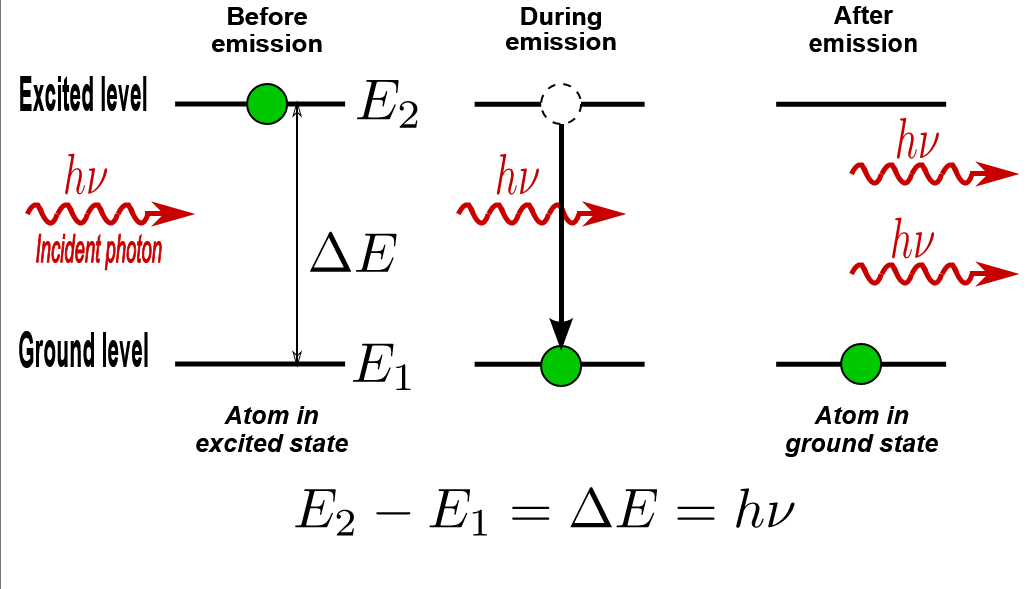
\includegraphics[width=0.3\textwidth]{Stim_Emission.png}
        
        \caption[width = 0.1\textwidth]{ Stimulated Emission  \cite{Laser_cav} }
        \label{fig:energy_diagram}
    \end{wrapfigure}
    \noindent The probability of a photon causing stimulated emission is equal to the probability of a photon falling to the ground state. $E_0$.
    This equality holds when the numbers of atoms in the ground and excited states are equal, resulting in a balanced rate of stimulated emission and absorption.
    By means of population inversion $N_2$/$N_1$ > 1, where $N_2$ is the population in the excited state and $N_1$ is the population in the ground state, the function of the laser is optimized.
    In other words, the population of the excited state must exceed that of the ground state.
    This allows for the production of a continuously increasing number of photons, establishing a higher output power for the laser medium.
    Understanding the interplay between absorption, stimulated emission, and population inversion is crucial for the design and operation of laser systems.
    By harnessing stimulated emission and achieving population inversion, lasers can produce a coherent light source. \cite{Laser_cav}
    %\monofig{width = 0.5\textwidth}{Stim_Emission.png}{ Stimulated Emission  \cite{Laser_cav} }{fig:energy_diagram}

\subsubsection{Pulsed Lasers (Mode Locking)}
    % Describe pulsed lasers, their advantages, and limitations.
    % Discuss the concept of time-bandwidth limit and its relevance.
    In order to generate ultra-short pulses of light in the range of picoseconds or femtoseconds, an optics technique called Mode Locking is used.
If the length of the laser's optical cavity is a multiple of the laser's fundamental frequency, standing waves or modes arise.
By fixing the phase relationship between the longetudinal modes, constructive interference between the standing waves is achieved, which produces synchronized pulses.
This method, known as mode locking, alters the behavior of the laser's modes, causing them to periodically constructively interfere and emit intense bursts of light.
The pulse duration is determined by the number of locked modes and their frequency separation, which is governed by the laser's spectral width.
    
\subsection{Second Harmonic Generation (SHG)}
    % Introduce SHG as a nonlinear optical process.
    % Explain how crystals generate light at twice the input frequency.
    % Discuss the importance of phase matching.
    %Second-harmonic generation (SHG), or frequency doubling, is a fundamental nonlinear optical process where two photons with the same frequency interact in a nonlinear material, combining to generate a new photon with double the energy.
    %This results in a photon with twice the frequency and half the wavelength of the initial photons,
    Second-harmonic generation (SHG) is a nonliniar optical process ,which is characterized by the second-order nonliniar susceptibility $\chi^{2}$ of a optical medium.
    In systems in which $\chi^{2}$ is non vanishing, two photons with the same frequency interact to form a photon with double the frequency and half the wavelength.
    To archieve high conversion rates the phase velocities of the incident wave and SH wave must be equal. \cite{demtroder2014laser}
     
    \begin{wrapfigure}[7]{r}[0cm]{0.4\textwidth}
        \centering
        \vspace{-\normalbaselineskip}
        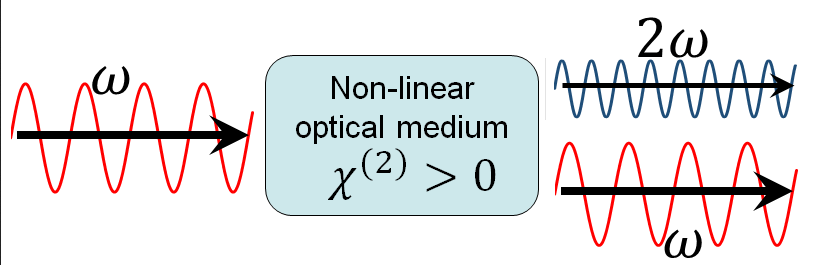
\includegraphics[width=0.4\textwidth]{shg_schem.png}
        \vspace{-10pt}
        \caption{Second harmonic generation \cite{shg}  }
        
        \label{fig:shg:basic}
    \end{wrapfigure}
    In negative birefringent uniaxial crystals, this is done by rotating the crystal in a certain direction where the extraordinary refractive index $n(2\omega)$ of the SH wave is equal to the ordinary refractive index $n(\omega)$ of the fundamental wavelength.
    The polarization direction of the SH wave is therefore orthogonal to that of the fundamental wave.
    For positive birefringent uniaxial crystals, it is switched, which means that the SH wave travels as an ordinary wave outside the medium.
    %conserving excitation coherence. SHG is utilized extensively, particularly in doubling laser frequencies, and is governed by the second-order nonlinear susceptibility of the medium. 
    %While SHG is typically prohibited in media with inversion symmetry, exceptions exist, such as in non-centrosymmetric crystals. 
    %Achieving efficient SHG often requires intense pulsed laser beams passing through large crystals with precise alignment for phase matching.

\subsection{Iodine Absorption \& Concentration}
    % Cover the absorption properties of iodine, including rotation, vibration, and temperature dependence.
    % Explain natural linewidth and temperature broadening effects.

Molecular iodine, which in the experiment described in the present document is examined in the gas phase as a diatomic molecule, exhibits absorption properties in the visible spectral range. These absorption properties, on one hand, arise due to the vibrational and rotational structure and the corresponding degrees of freedom of such molecules. On the other hand, electronic state transitions from ground states to excited states enable further absorption of specific wavelengths in the visible range \cite{demtroder2014laser}.

The absorption lines apparent in the absorption spectrum are expected to be slim and narrowly centered around the characteristic wavelengths corresponding to valid state transitions. There are a number of effects that lead to the broadening of these spectral lines, most importantly the intrinsic natural broadening arising from the finite lifetime of excited states. A second important effect is called temperature broadening, which results from the thermal motion of particles due to the Doppler effects. The latter effect only becomes apparent at high temperatures of the sample however \cite{demtroder2014laser}.

The decadic absorbance $A$ is described by
\begin{equation}
    \label{eq:fundamentals:absorbance}
    A = \log_{10}\left(\frac{I_0}{I_t}\right) ,
\end{equation}
where $I_0$ is the measured laser intensity without iodine and $I_t$ is the intensity transmitted by the iodine \cite{demtroder2014laser}. For small molar concentrations $c$, the Lambert-Beer law relates the absorbance $A$ to the effective interaction length $l$ of the laser beam with the iodine and the molecular absorption coefficient $\varepsilon$ as follows \cite{attenuation}.
\begin{equation}
    \label{eq:fundamentals:beer}
    A = l \cdot c \cdot \varepsilon
\end{equation}

The absorption cross-section $\sigma$ of iodine, which is a measure for the probability of an absorption process, commonly denoted in units of \si{\cm\squared\per\molecule} and available in scientific literature such as \cite{Iodine}, can be used to obtain the molecular absorption coefficient $\varepsilon$ via the relation
\begin{equation}
    \label{eq:fundamentals:absorptivity}
    \sigma = \frac{\ln(10) \cdot 10^3}{N_A} \cdot \varepsilon ,
\end{equation}
where $N_A$ is the Avogadro Constant \cite{attenuation}. The molecular absorption coefficient is commonly specified in units of \si{\liter\per\mol\per\cm} and - contrary to the absorbance $A$ - uses $e$ as logarithmic base, explaining the need for the term $ln(10) \cdot 10^3$ in Equation \ref{eq:fundamentals:absorptivity} due to base and unit conversion.


\subsection{Grating Spectrometer}
% Briefly mention grating spectrometers and their role in analyzing laser spectra.
% Explain how diffraction gratings disperse light for spectral measurements.

Spectrometers in general are optical instruments that create images which are laterally separated for different wavelengths $\lambda$ of the incident radiation. In the case of a grating spectrometer, as opposed to spectral dispersion used in a prism spectrometer, the lateral dispersion is due to diffraction plane or concave reflection gratings \cite{demtroder2014laser}.
\begin{wrapfigure}[14]{r}[0cm]{0.4\textwidth}
    \centering
    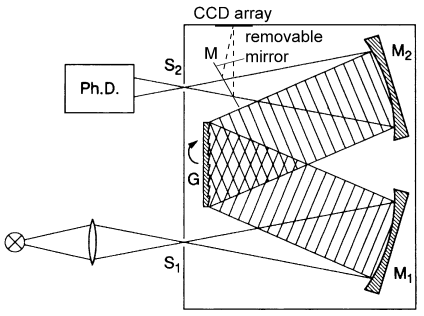
\includegraphics[width=0.3\textwidth]{graphics/spectrometer.png}
    
    \caption[width = 0.1\textwidth]{Schematic structure of a grating spectrometer \cite{demtroder2014laser}.}
    \label{fig:fundamentals:spectrometer}
\end{wrapfigure}
In a grating spectrometer as shown in Figure \ref{fig:fundamentals:spectrometer}, the light source illuminates the entrance slit $S_1$, which is in the focal plane of a spherical mirror $M_1$. The collimated, parallel light is reflected by $M_1$ onto a reflection grating consisting of many straight grooves parallel to the entrance slit. Highly reflective metal or dielectric coating on the surface of the grating is used to reflect the light towards a second spherical mirror $M_2$,which in turn focuses it onto the exit slit $S_2$ or onto a photographic plate in the focal plane of $M_2$ \cite{demtroder2014laser}.

%\begin{figure}[H]
%    \centering
%    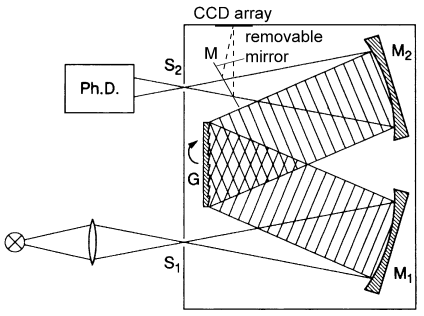
\includegraphics[width=0.45\textwidth]{graphics/spectrometer.png}
%    \caption{Schematic structure of a grating spectrometer \cite{demtroder2014laser}.}
%    \label{fig:fundamentals:spectrometer}
%\end{figure}

\noindent Considering the coherently illuminated grooves on the grating as individual sources of radiation, each of them diffracting the incident light into a larger range around the direction nof geometrical reflection, the resulting outgoing intensity is subject to destructive and constructive interference, where for the latter the grating equation is
\begin{equation}
    \label{eq:fundamentals:grating}
    2 d \cdot \sin(\alpha) = m \lambda ,
\end{equation}
where $d$ is the width of each groove and $\alpha$ is the angle of the $m$-th order maximum at incident wavelength $\lambda$ \cite{demtroder2014laser}. From Equation \ref{eq:fundamentals:grating} follows the spectral resolving power as
\begin{equation}
    \label{eq:fundamentals:resolving}
    R = \frac{\lambda}{\Delta \lambda} = m N ,
\end{equation}
for diffraction order $m$ with the total number $N$ of illuminated grooves \cite{demtroder2014laser}.

While using a prism spectrometer would have the advantage of unambiguous assignment of wavelengths $\lambda$, which is not the case for grating spectrometers due to a diffraction pattern with potentially overlapping orders of diffraction being produced, the former offer only moderate spectral resolution compared to grating spectrometers. Also, since the current experiment involves infrared radiation, for which coated mirrors and gratings exhibit especially high reflectivity, grating spectrometers are preferred over prism spectrometers in such scenarios \cite{demtroder2014laser}.

\newpage
%************VERSUCHSANORDNUNG*************
\section{Setup}
\label{sec:setup}


\begin{figure}[H]
    \centering
    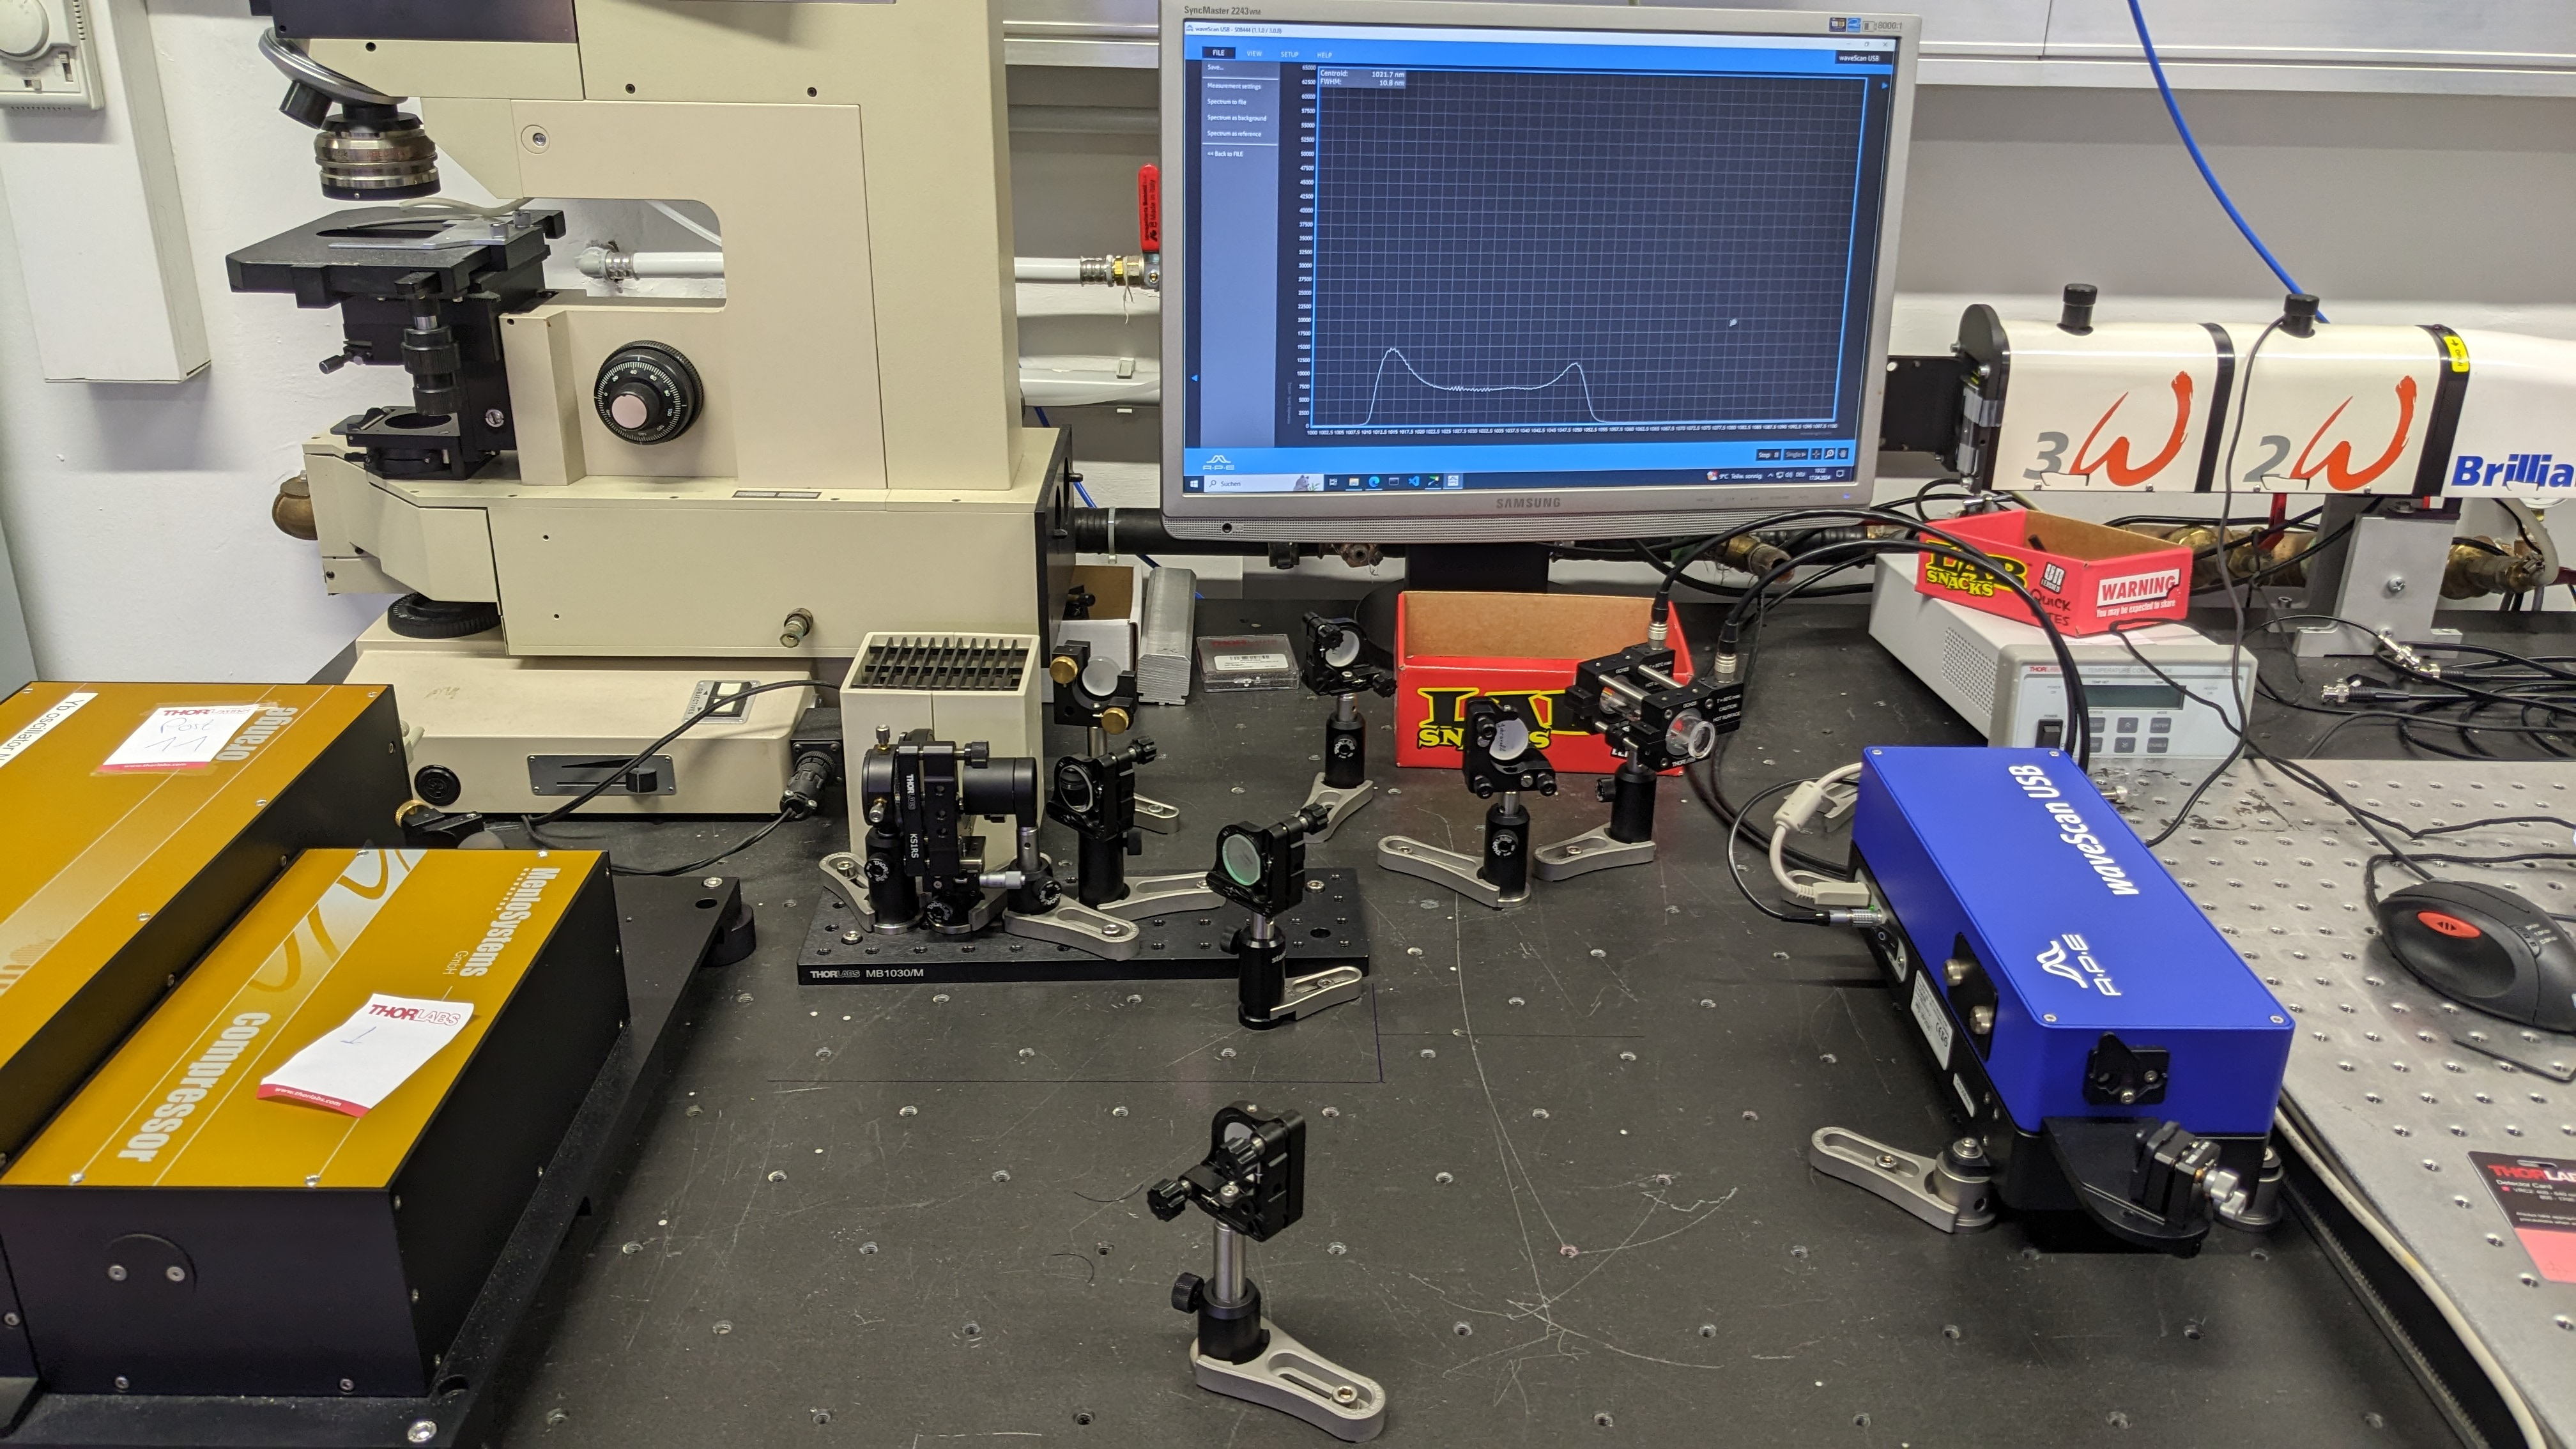
\includegraphics[width=0.1\textwidth]{graphics/basic-setup.jpg}
    \caption{basic snoop}
    \label{fig:setup:basic}
\end{figure}
%************GERÄTELISTE***************
\section{Equipment}
\label{sec:equipment}
\begin{table}[H]
	\centering
	\caption{
		Devices and utensils used in the experiment.
		}
	\begin{tabular}[h]{| l | l | l | l |}
		\hline
		Device     & Manufacturer   & Model  & tech. Data / Uncertainty       \\\hline
		\hline
		Power Meter & Thorlabs & PM100D & \cite{Power} \\ \hline
		Grating Spectrometer & APE & Wavescan USB &  \cite{Speck} \\ \hline
		Yb Laser & Menlosystems & Femtosecond Ytterbium Laser & \cite{Laser} \\ \hline
		3x Dielectric Mirrors & Thorlabs & BB1-E02 & 400 - 750 nm \\ \hline
		2x Dielectric Mirrors & Thorlabs & BB1-E03 & 750 - 1100 nm \\ \hline
		Iodine Cell & - & - & - \\ \hline
 		Temperature Controller & Thorlabs & TC200 & \cite{TempC} \\ \hline
		Collimator &Thorlabs & - &- \\ \hline 
		Collecting Lens & Thorlabs & -& - \\ \hline
		SHG - Crystal & - & - & - \\ \hline
	\end{tabular}
	\label{tab:Geraeteliste}
\end{table}
\newpage
%************VERSUCHSDURCHFÜHRUNG & MESSERGEBNISSE***********
\section{Execution}
\label{sec:execution}

This sections serves as documentation on how the results as described in Section \ref{sec:summary} might be reproduced. Instructions are based on the assumption that an environment with suitable equipment such as described in Sections \ref{sec:setup} and \ref{sec:equipment} is used and set up accordingly.

\subsection{Laser Source and Safety}
\label{sec:laser-source-and-safety}

All experimental steps described in subsequent sections require the infrared laser source to be operational, for which the main switch needs to be activated. Additionally, there is a cover at the output of the laser source blocking the outgoing beam that needs to be opened during measurement.

For safety reasons, this cover is to remain closed while changes to the setup are made. Furthermore, safety goggles need to be used and reflective apparel such as watches or rings need to be removed. The eyes of the experimentators must strictly remain well above the path of the laser beams.

\subsection{Beam Positioning}
\label{sec:execution:beam-positioning}

For the laser beam to be measured by the grating spectrometer, it needs to be directed from the output of the laser source towards the input aperture of the spectrometer. This is achieved by directing it via a series of dielectric mirrors, which are positioned and aligned such that on one hand the SHG stage and the iodine cell can be traversed by the beam, while on the other hand the beam reaches the aperture of the spectrometer in a correct angle.

For a wavelength of \SI{1030}{\nm}, the mirrors of type E03 are used, while for beams after the SHG stage with a desired wavelength of \SI{515}{\nm} the type E02 mirrors are utilised. Using the latter for beams in the visible green spectrum ensures that a portion of remaining infrared photons are not reflected, effectively filtering them on the way to the spectrometer.

As described in Section \ref{sec:setup}, the bases for the optical elements used in this experiment can be positioned and fixed on a grid of tapped holes. While the bases allow for vertical adjustment as well as crude rotation with respect to the vertical axis, the mounts allow for fine-tuned vertical and horizontal tilting of the mirrors, thus enabling alignment of the laser beam as desired.

One strategy that proves to be advantageous is to locate the mirrors in such a way that the beam follows a path containing only angles of approximately \SI{90}{\degree}, for which the reflection angle relative to each mirror is approximately \SI{45}{\degree}. For this approach the grid of tapped holes in the table can be used as a rough reference, while additionally the sensitivity for changes in mirror angle are minimized.

As shown in Figure \ref{fig:execution:aperture}, the grating spectrometer exhibits a dedicated adjustable mirror for directing the laser beam towards the aperture. There are covers at both the mirror and the aperture, each containing a special hole to be used for properly adjusting the laser beam while the covers are closed. When correctly adjusted, the laser beam hits both the hole at the mirror as well as the hole at the cover of the aperture. During measurement, the cover at the mirror is always to be opened.

\begin{figure}[H]
    \centering
    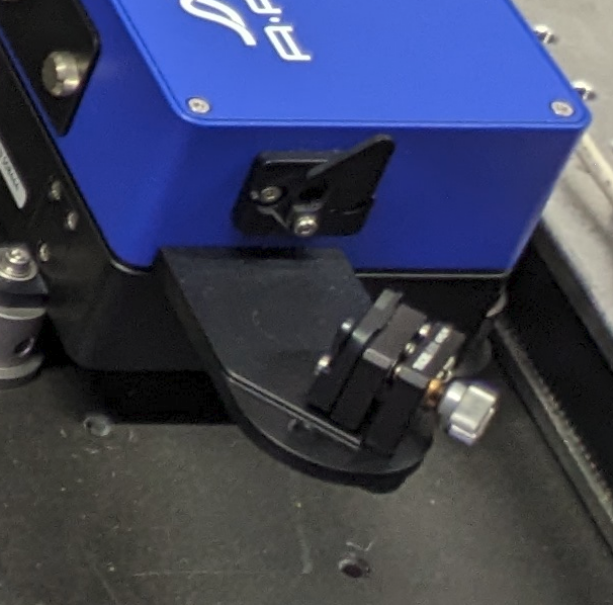
\includegraphics[width=0.45\textwidth]{graphics/aperture.png}
    \caption{Aperture and dedicated mirror at the grating spectrometer.}
    \label{fig:execution:aperture}
\end{figure}

The overall procedure for directing the beam towards the spectrometer as desired involves stepwise adjustment of the mirrors starting from the laser source and going towards the spectrometer, followed by iterative fine-tuning of each mirror both in height and rotation.

\subsection{Measurement Procedure}
\label{sec:execution:measurement-procedure}

In order to measure the power of the beam, the power meter as documented in Table \ref{tab:equipment} and depicted in Figure \ref{fig:execution:powermeter} is used. The photodiode sensor needs to be connected to the console via cable and placed such that it is hit by the laser beam. For all measurements described in the subsequent sections, the relative measurement mode is activated by pressing the "$\Delta$" button. While the range is always set to automatic mode, the wavelength is set manually to either $\SI{1030}{\nm}$ for the infrared laser or $\SI{515}{\nm}$ for the frequency-doubled laser, which can be achieved by navigating the menu using the arrow and "OK" buttons. It should be noted here that setting the wavelength is merely used for calculating the power - the power meter does not filter unrelated wavelengths.

\begin{figure}[H]
    \centering
    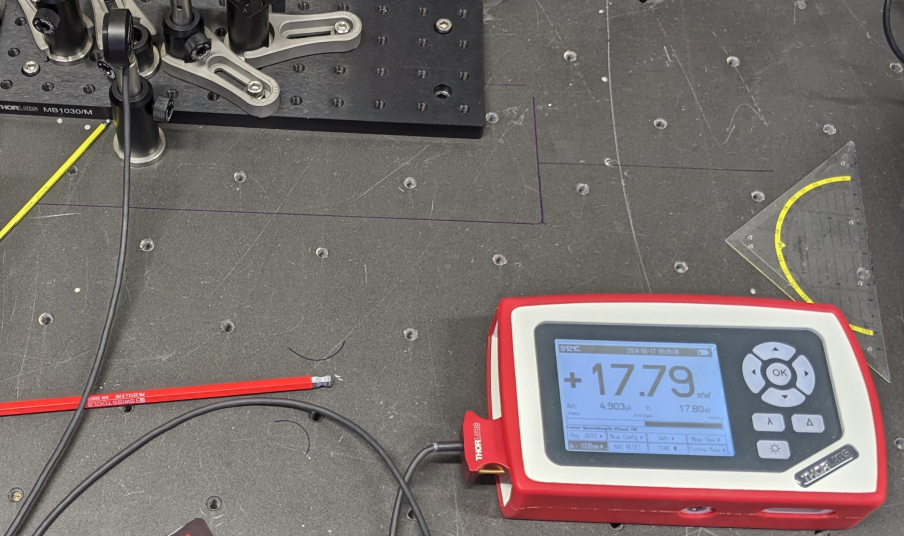
\includegraphics[width=0.45\textwidth]{graphics/power-meter.png}
    \caption{Power meter consisting of console and sensor.}
    \label{fig:execution:powermeter}
\end{figure}

For the grating spectrometer, which needs to be set up as described in Section \ref{sec:execution:beam-positioning}, measurement needs to be started by clicking the "Start" button in the bottom right corner. The view of the measured spectrum is updated in realtime and can be zoomed in by clicking the magnifying glass button or reset via the crosshair button, which are both located in the bottom right corner of the user interface.

The "View" and "Setup" menus in the top left corner of the interface allow to enable averaging of the measured spectra for up to $256$ measurements, which proves beneficial for reducing noise. The menus also allow to confine the wavelength of the spectra to a specific domain, increasing the available resolution when considering specific regions of interest.

For exporting measured spectra, the "File$~$\textrightarrow$~$Spectrum to file" operations are used. It is important to notice that the used version of the software as documented in Table \ref{tab:equipment} updates the data until the instant where the "Save" button in the file dialog is being hit. Using "File$~$\textrightarrow$~$Spectrum as reference" an existing spectrum may be loaded, which in addition to the spectrum currently measured will be displayed in the user interface. This allows to visually compare current measurements with previously recorded spectra for reference.

\begin{figure}[H]
    \centering
    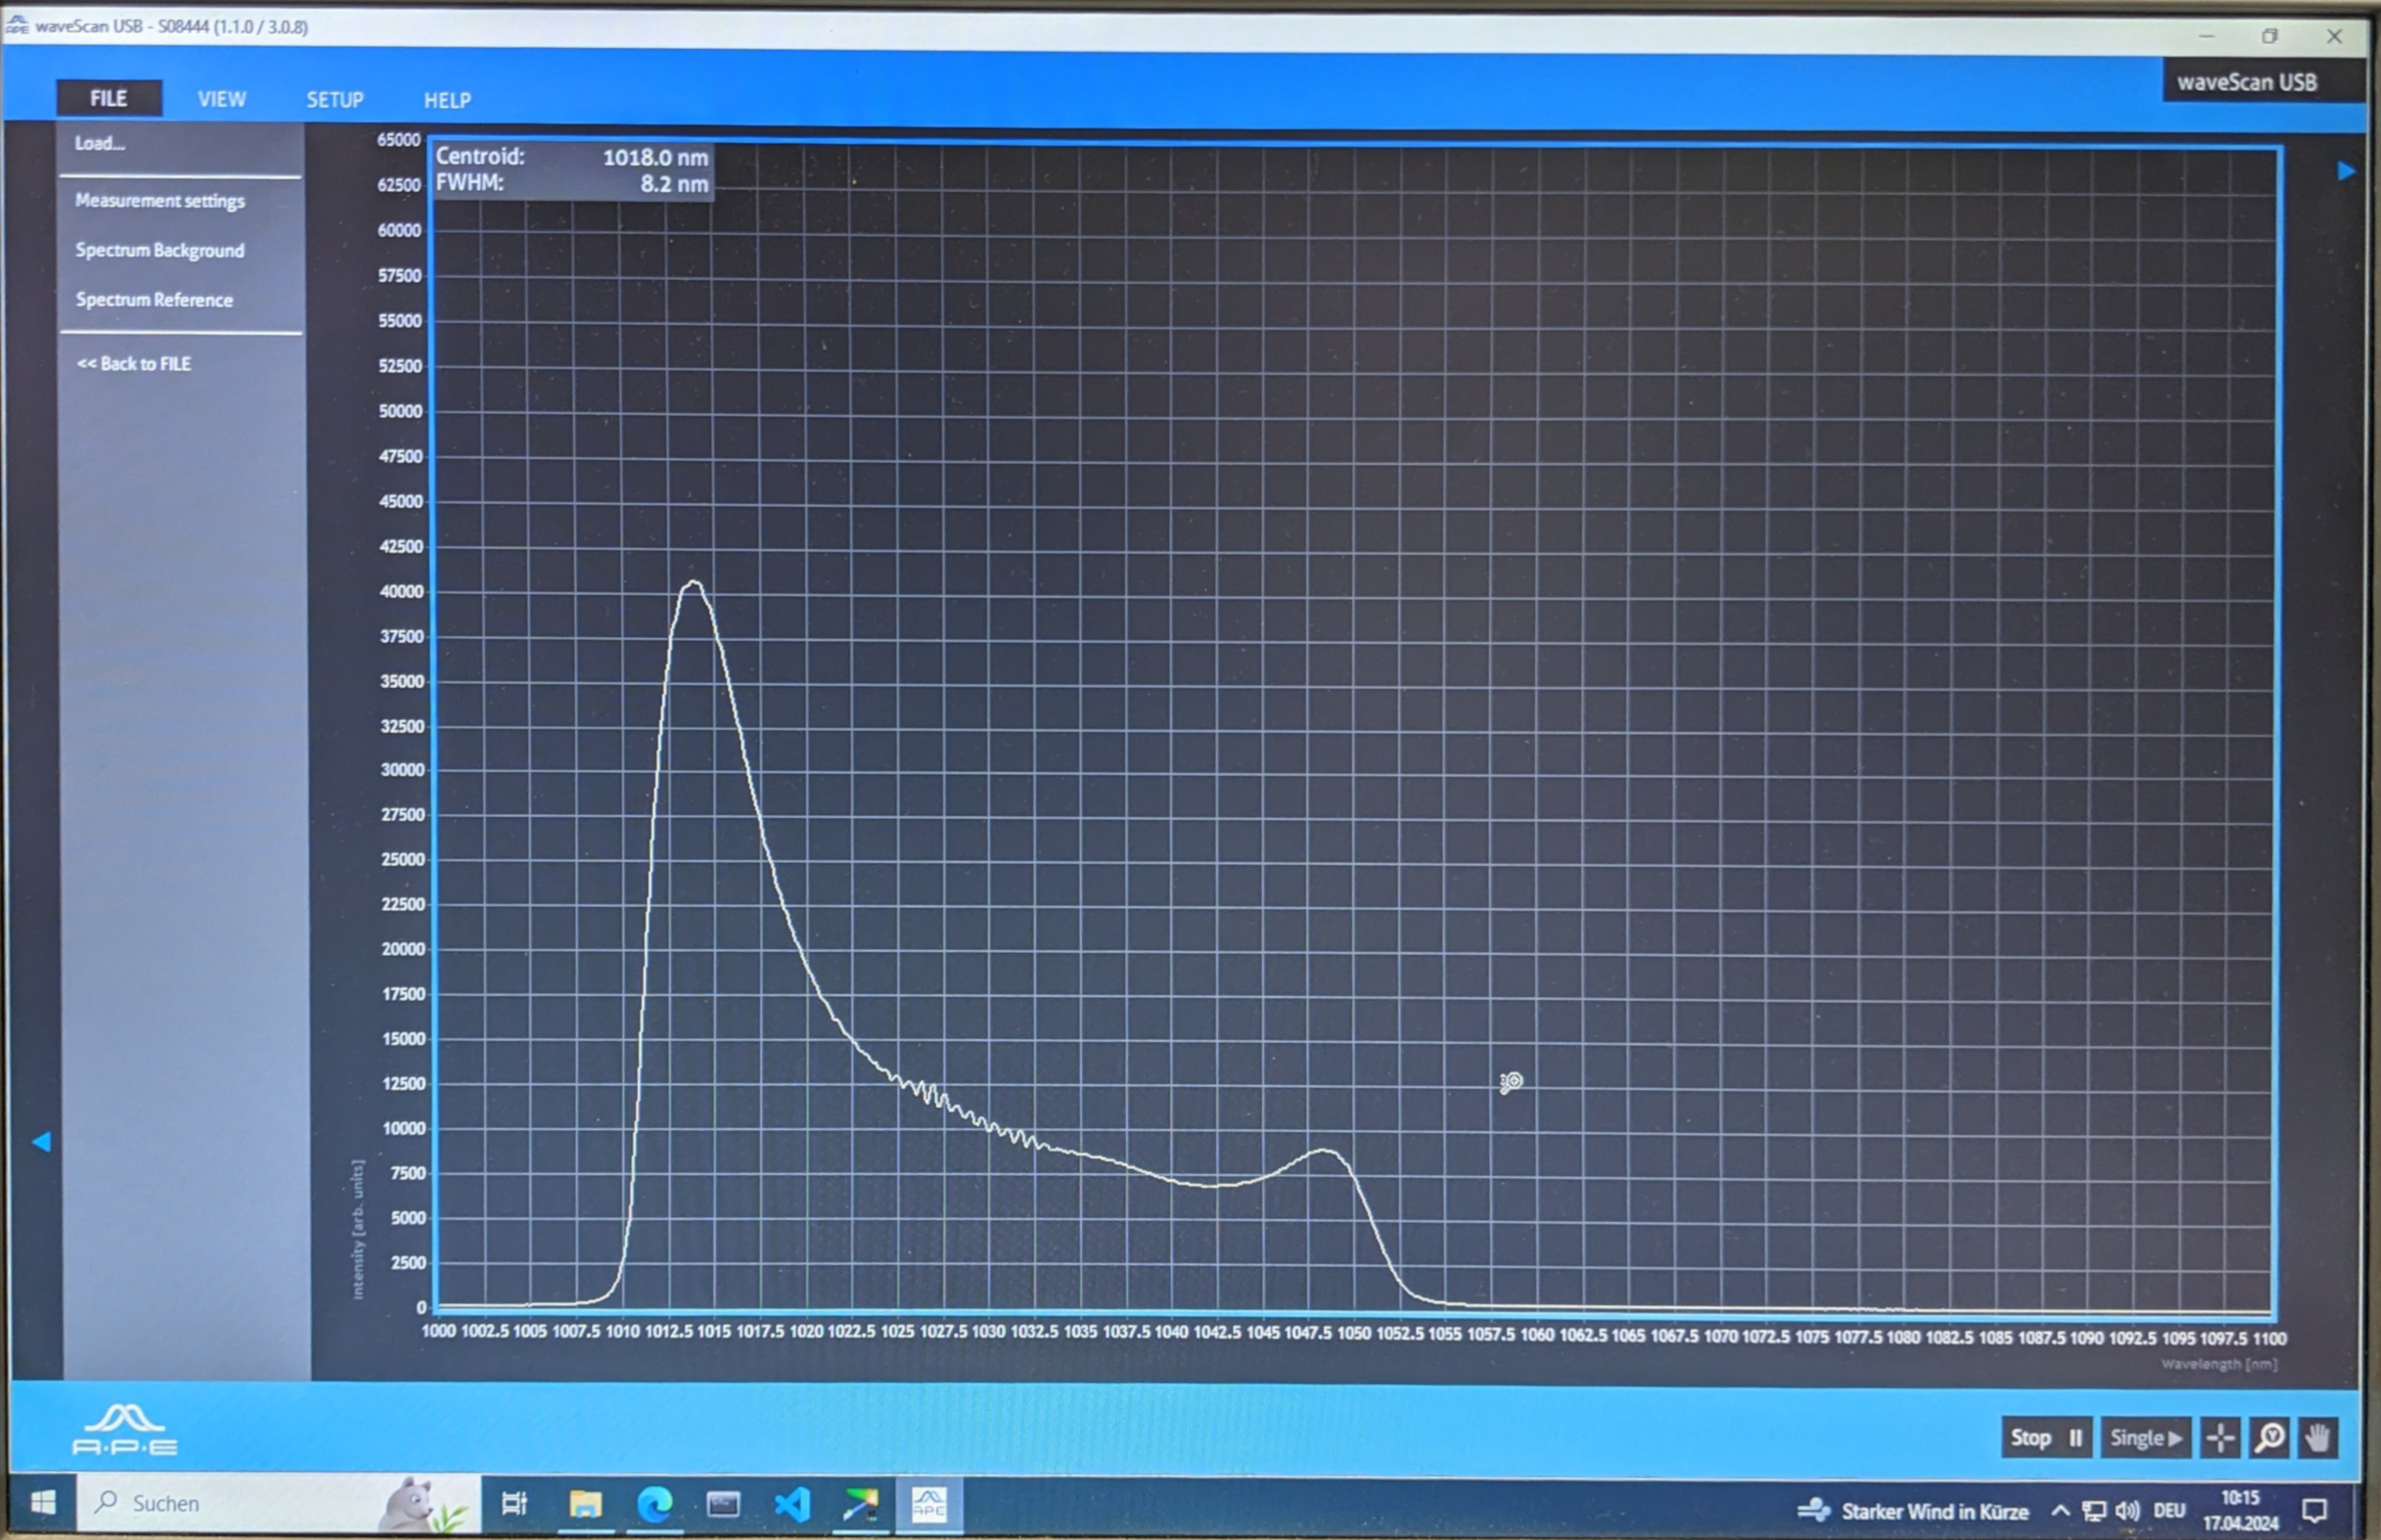
\includegraphics[width=0.45\textwidth]{graphics/wave-scan.jpg}
    \caption{Graphical interface of APE waveScan.}
    \label{fig:execution:wave-scan}
\end{figure}

\subsection{Laser Source Characterization}
\label{sec:execution:infrared-characterization}

In a first step, the infrared laser beam emitted by the laser source is characterized. As depicted in Figure \ref{fig:setup:power}, operating as described in sections \ref{sec:execution:beam-positioning} to \ref{sec:execution:measurement-procedure}, the average power output is measured for a wavelength of \SI{1030}{\nm} using the power meter. Taking into account the uncertainty of the photodiode sensor as documented in Table \ref{tab:equipment}, which is specified as $\pm \SI{7}{\percent}$ in the used range, and further considering deviations of the laser source from the wavelength of \SI{1030}{\nm} used by the console for calculating the power, a combined uncertainty of $\pm \SI{10}{\percent}$ is assumed. The average power of the infrared source therefore reads $P_{IR} = \SI{17.8(18)}{\mW}$.

In order to be able to obtain the central wavelength as well as FWHM of the infrared laser, the spectrometer is used to measure and export the spectrum in a format such as shown in Table \ref{tab:execution:infrared-characterization}. For this, the procedure as described in sections \ref{sec:execution:beam-positioning} to \ref{sec:execution:measurement-procedure} is followed. The setup for obtaining the spectrum is shown in Figure \ref{fig:setup:basic}.

\begin{table}[H]
    \centering
    \caption{Intensity spectrum for the infrared laser. \\
    $\lambda$ = Wavelength, $I$ = Intensity count}
    \label{tab:execution:infrared-characterization}
    \begin{tabular}{ccccc}
    \hline
    $\lambda$ / nm & $I$ / 1 \\ \hline
    1000  & 28  \\
    \vdots & \vdots  \\
    1100 & 216 \\ \hline
    \end{tabular}
\end{table}

\subsection{SHG Characterization}
\label{sec:execution:shg-characterization}

In a second step, the SHG stage, which is described in more detail in Section \ref{sec:setup}, is added to the setup as shown in Figure \ref{fig:setup:shg}. This involves proper re-alignment of the beam path using type E02 mirrors, which is described in Section \ref{sec:execution:beam-positioning}, as well as adjustment of all optical elements of the SHG. 

Rotating the non-linear crystal such that phase matching required for successful SHG is achieved and based on this the amount of frequency-doubled photons is maximized is of particular importance. Rotation of the crystal is conveniently afforded by the corresponding mount.

Analogous to the procedure in Section \ref{sec:execution:infrared-characterization}, the power meter is used to obtain the average power of the green laser beam. After configuring the wavelength of \SI{515}{\nm} at the console, for which the photodiode sensor specifies an uncertainty of $\pm \SI{3}{\percent}$, and further considering significant deviations of the SHG output from the wavelength of \SI{515}{\nm} (including remaining infrared photons) used by the console for calculating the power, a combined uncertainty of $\pm \SI{15}{\percent}$ is assumed. The average power of the SHG source therefore reads $P_{SHG} = \SI{3.7(6)}{\mW}$.

The spectrometer is used to obtain and export the spectrum just as described in Section \ref{sec:execution:infrared-characterization}. The resulting data is shown in Table \ref{tab:execution:shg-characterization}.

\begin{table}[H]
    \centering
    \caption{Intensity spectrum for the SHG output. \\
    $\lambda$ = Wavelength, $I$ = Intensity count}
    \label{tab:execution:shg-characterization}
    \begin{tabular}{ccccc}
    \hline
    $\lambda$ / nm & $I$ / 1 \\ \hline
    500  & 10.6  \\
    \vdots & \vdots  \\
    530 & 16.6 \\ \hline
    \end{tabular}
\end{table}

\subsection{Iodine Absorbance}
\label{sec:execution:iodine}

In order to investigate iodine absorbance, the iodine cell as described in Table \ref{tab:equipment} is added to the beam path of the setup used in Section \ref{sec:execution:shg-characterization} in such a way that the SHG output traverses the iodine cell. This new setup is shown in Figure \ref{fig:setup:iodine}, where also two additional type E02 mirrors are added in order to triple the interaction length of the beam with the iodine gas. Alignment of all optical elements is as always done as described in Section \ref{sec:execution:beam-positioning}. 

Additionally, the iodine cell is connected to two heating elements connected to the temperature controller shown in Figure \ref{fig:setup:temperature-controller}. After activating the controller, it becomes obvious that at approximate room temperature of \SI{23}{\celsius} the temperature displayed is \SI{29.6}{\celsius}, resulting in an approximate shift of \SI{7}{\celsius} to be taken into account for future considerations. Given these circumstances as well as the specified uncertainty of the temperature controller of $\pm \SI{0.5}{\celsius}$ according to Table \ref{tab:equipment}, the temperature readings are decreased by \SI{7}{\celsius} and equipped with a combined uncertainty of $\pm \SI{3}{\celsius}$.

Analogous to the procedure described in Section \ref{sec:execution:shg-characterization}, the spectra are recorded and exported for a single-pass configuration at three temperatures in the range of \SI{20}{\celsius} to \SI{60}{\celsius}. The corresponding data is shown in tables \ref{tab:execution:iodine:single:1} to \ref{tab:execution:iodine:single:3}. Additionally, at approximately \SI{60}{\celsius} the spectrum is recorded for the triple-pass configuration. The corresponding data is shown in Table \ref{tab:execution:iodine:triple}. For all measurements, an averaging setting of $100$ is applied.

\begin{figure}[H]
    \centering
    \begin{minipage}[b]{0.48\textwidth}
        \centering
        \begin{table}[H]
            \centering
            \caption{Iodine spectrum at \SI{23(3)}{\celsius} \\in single-pass configuration. \\
            $\lambda$ = Wavelength, $I$ = Intensity count}
            \label{tab:execution:iodine:single:1}
            \begin{tabular}{ccccc}
            \hline
            $\lambda$ / nm & $I$ / 1 \\ \hline
            505  & 17.1  \\
            \vdots & \vdots  \\
            525 & 22.2 \\ \hline
            \end{tabular}
        \end{table}
    \end{minipage}
    \hfill
     \begin{minipage}[b]{0.48\textwidth}
        \centering
        \begin{table}[H]
            \centering
            \caption{Iodine spectrum at \SI{35(3)}{\celsius}. \\in single-pass configuration. \\
            $\lambda$ = Wavelength, $I$ = Intensity count}
            \label{tab:execution:iodine:single:2}
            \begin{tabular}{ccccc}
            \hline
            $\lambda$ / nm & $I$ / 1 \\ \hline
            505  & 12.7  \\
            \vdots & \vdots  \\
            525 & 25.1 \\ \hline
            \end{tabular}
        \end{table}
    \end{minipage}
\end{figure}

\begin{figure}[H]
    \centering
    \begin{minipage}[b]{0.48\textwidth}
        \centering
        \begin{table}[H]
            \centering
            \caption{Iodine spectrum at \SI{53(3)}{\celsius}. \\in single-pass configuration. \\
            $\lambda$ = Wavelength, $I$ = Intensity count}
            \label{tab:execution:iodine:single:3}
            \begin{tabular}{ccccc}
            \hline
            $\lambda$ / nm & $I$ / 1 \\ \hline
            505  & 18.0  \\
            \vdots & \vdots  \\
            525 & 23.3 \\ \hline
            \end{tabular}
        \end{table}
    \end{minipage}
    \hfill
     \begin{minipage}[b]{0.48\textwidth}
        \centering
        \begin{table}[H]
            \centering
            \caption{Iodine spectrum at \SI{53(3)}{\celsius}. \\in triple-pass configuration. \\
            $\lambda$ = Wavelength, $I$ = Intensity count}
            \label{tab:execution:iodine:triple}
            \begin{tabular}{ccccc}
            \hline
            $\lambda$ / nm & $I$ / 1 \\ \hline
            505  & 13.8  \\
            \vdots & \vdots  \\
            525 & 20.0 \\ \hline
            \end{tabular}
        \end{table}
    \end{minipage}
\end{figure}

\subsection{Iodine Cell Dimensions}
\label{sec:execution:iodine-cell-dimensions}

Using the set square specified in Table \ref{tab:equipment}, the dimensions of the iodine cell are measured. Given a slant-cut cylindrical cell such that a cross-section along the axis is trapezoid-shaped, the longer base is measured to be of length $l_l = \SI{98(2)}{\mm}$ and the shorter base of length $l_s = \SI{90(2)}{\mm}$ respectively. The uncertainties specified are a suitably chosen combined uncertainty consisting of inaccuracies inherent to the manufacturing of the set square as well as parallax effects and subjective reading uncertainties. Both $l_l$ and $l_s$ consider the thickness of the slant areas and describe the shortest and longest possible path in pure iodine gas respectively.

\newpage
%************AUSWERTUNG****************
\section{Evaluation}
\label{sec:evaluation}

For evaluation purposes, the scripting language \verb|Python| \cite{PYTHON} is utilized.
The Python libraries, \verb|numpy| \cite{harris2020array}, \verb|pandas| \cite{reback2020pandas}, \verb|scipy| \cite{2020SciPy-NMeth} and \verb|matplotlib| \cite{Hunter:2007} are used for statistical calculation operations, reading and processing data and creating plots.

Unless specified otherwise, the maximum uncertainty method according to Equation \ref{equ:groestunsicherheit} \cite{MMETH} is used for all uncertainty calculations.
For this purpose, the total differential of the outgoing equation is formed and the absolute values of the summands are multiplied by the uncertainty determined.
Statistical evaluations are subject to a statistical uncertainty according to the Student-t distribution.
\begin{equation}
    \varDelta f = \biggl| \frac{\partial f}{\partial x_{1}} \cdot \varDelta x_{1} \biggl| + \biggl| \frac{\partial f}{\partial x_{2}} \cdot \varDelta x_{2} \biggl| + .... + \biggl| \frac{\partial f}{\partial x_{n}} \cdot \varDelta x_{n} \biggl|
    \label{equ:groestunsicherheit}
\end{equation}

In the present evaluation, the library \verb|uncertainties| \cite{UN} is used for calculating any uncertainty propagation, as this is based on the principle of the maximum uncertainty method as described in Equation \ref{equ:groestunsicherheit}.

\subsection{Laser Source Characterization}
In order to obtain the central wavelength and the full width half maximum $FWHM$, the data obtained as described in Section \ref{sec:execution:infrared-characterization} is fitted using the function \verb|curve_fit|.
The measured IR spectra are fitted using a sum of multiple gaussian distributions,as seen in Equation \ref{eq:evaluation:fitfunc}.
For convenience, the spectra were divided by the maximum value of the emission lines. 
\begin{equation}
    G_{comb}(\lambda) = \sum_{p = 1} A_p e^{-\frac{(\lambda - \lambda_p)^{2}}{2 \sigma_{p}^2}}  = \sum_{p = 1} G_p(\lambda)
    \label{eq:evaluation:fitfunc}
\end{equation}
Judging by the estimated parameters in Table \ref{tab:evaluation:ir_fitted1}, the emission spectrum of Ytterbium reduces to 7 individual lines, resulting in a bimodal structure.
The resulting function is then normalized by integrating over the defined space to get a power density.
Using Equation \ref{eq:evaluation:central}, the central wavelength $\langle \lambda \rangle$ is calculated by integrating over $\lambda G_{comb}(\lambda)$, where $G_{comp}$ is the superposition of gauss distributions. 

\begin{equation}
    \langle \lambda \rangle = \frac{1}{K} \int_{P}\lambda G_{comp}(\lambda) d \lambda
    \label{eq:evaluation:central}
\end{equation}
\monofig{width=\textwidth}{IR_fitted.pdf}{
    Emission spectra of Yb Laser and its fit function. \\
    $G_i(\lambda_p)$ = Gaussian fitfunctions with corresponding wavelengths $\lambda_p$ at peakpositions,
    $G_{comb}(\lambda)$ = Superposition of all gaussian fitfunctions,
    $\lambda_c$ = central wavelength,
    $FWHM_{total}$ = total full width half maximum
     }{fig:evaluation:ir_fitted}
The outer most peaks are used to estimate the FWHM by using the relation $FWHM = 2 \sqrt{2 \ln(2)} \cdot \sigma$, which holds for all Gauss distributions.
Now the distance between the two outermost FWHM points is calculated to estimate the total full width half maximum, $FWHM_{total}$, as seen in Figure \ref{fig:evaluation:ir_fitted}.
The error estimates for the fit function were calculated using the diagonal elements of the covariance matrix obtained by the library routine, which are an estimation for the variance of the fit parameters.
Further discussion regarding the results is in Section \ref{sec:discussion}.
\begin{table}[H]
\centering
\caption{
    Fitting Parameter Laser Source Characterization. \\
    $A_p$: Gaussian Amplitudes,
    $\lambda_p$: Expectation value,
    $\sigma_p$: Standart diviations,
    $G_p$: functions associated with the parameters,
}
\begin{tabular}{c|ccc} \hline
    &  $A_p$ / 1 &  $\lambda_p$ / nm & $\sigma_p$ / nm  \\ \hline  \hline 
$G_0$&$0.40 \pm 0.07$&$1012.37 \pm 0.04$&$1.03 \pm 0.05$\\ \hline
$G_1$&$0.63 \pm 0.13$&$1014.46 \pm 0.13$&$1.71 \pm 0.18$\\ \hline
$G_2$&$0.445 \pm 0.014$&$1025.25 \pm 0.26$&$5.52 \pm 0.41$\\ \hline
$G_3$&$0.46 \pm 0.08$&$1017.63 \pm 0.51$&$2.80 \pm 0.34$\\ \hline
$G_4$&$0.490 \pm 0.009$&$1038.46 \pm 0.24$&$5.89 \pm 0.22$\\ \hline
$G_5$&$0.43 \pm 0.04$&$1046.49 \pm 0.31$&$2.70 \pm 0.19$\\ \hline
$G_6$&$0.57 \pm 0.06$&$1049.50 \pm 0.03$&$1.69 \pm 0.05$\\ \hline
\end{tabular}
\label{tab:evaluation:ir_fitted1}
\end{table}
\newpage
\subsection{SHG Characterization}
Using the same methods as before, a fitting function is estimated, and afterwards the central wavelength is $\langle \lambda \rangle$.
The spectrum is again divided by the maximum intensity for convenience in fitting.
As the individual peaks are quite well resolved, it would not make sense to estimate the FWHM, and therefore only the individual FWHM is calculated.
The peaks from the residual IR spectrum align nicely with the SHG spectrum if one divides them by two, which is expected with the phonomena of frequency doubling.
Also, the central wavelength of the SHG spectrum is almost exactly half of the residual IR spectrum.
More so, the SHG spectrum suggests that some of the incoming IR wavelengths are preferred over others for SH generation.

\duofigcom{SHG_fitted_better1.pdf}{fig:evaluation:greenfitted}{SHG_fitted_better2.pdf}{fig:evaluation:redfitted}{
    (a) Second Harmonic Generation spectrum. (b) Residuel Spectrum \\
    $G_i(\lambda_p)$ = Gaussian fitfunctions with corresponding wavelengths $\lambda_p$ at peakpositions,
    $G_{comb}(\lambda)$ = Superposition of all gaussian fitfunctions,
    $\lambda_c$ = central wavelength,
    }
    {fig:evaluation:shg_fitted}
\noindent The residual IR spectrum has substantially more noise than the other spectra because its maximal intensity is so low.
This results in less precise fitting and a long parameter convergence time.
To get the conversion rate $C$ first the fitting function of the SHG spectrum is integrated over the relevant interval around the peaks. 
Then it is divided by the sum of the two fitting functions in Figure \ref{fig:evaluation:shg_fitted} and integrated under the assumption of energy conservation.:
    
\begin{align}
    CR &= \frac{\int_{\varOmega} G_{SHG}(\lambda) d \lambda}{ \int_{\Sigma} (G_{SHG}(\lambda) + G_{IR}(\lambda))d \lambda} \\
    CR &= (0.84 \pm 0.02)  \hspace{2pt} \% \hspace{3cm} CR \ldots \text{Conversionrate}
\end{align}

\begin{table}[H]
    \label{}
    \centering
    \caption{Fitting Parameter SHG Spectrum. \\
    $A_p$: Gaussian amplitudes,
    $\lambda_p$: Expectation value,
    $\sigma_p$: Standart diviations,
    $G_p$: functions associated with the parameters,}
    
    \begin{tabular}{c|ccc} \hline
        &  $A_p$ / 1 &  $\lambda_p$ / nm & $\sigma_p$ / nm \\ \hline \hline 
    $G_0$&$0.39 \pm 0.02$&$509.85 \pm 0.13$&$1.48 \pm 0.06$\\ \hline
    $G_1$&$0.80 \pm 0.04$&$511.53 \pm 0.01$&$0.79\pm 0.02$\\ \hline
    $G_2$&$0.49 \pm 0.01$&$514.40 \pm 0.01$&$0.44 \pm 0.01$\\ \hline
    $G_3$&$0.11 \pm 0.01$&$517.95 \pm 0.04$&$0.73 \pm 0.04$\\ \hline
    $G_4$&$0.20 \pm 0.01$&$521.98 \pm 0.03$&$1.26 \pm 0.03$\\ \hline
    \end{tabular}
    \end{table}

\begin{table}[H]
        \label{}
        \centering
        \caption{Fitting Parameter Residual Spectrum. \\
        $A_p$: Gaussian amplitudes,
        $\lambda_p$: Expectation value,
        $\sigma_p$: Standart diviations,
        $G_p$: functions associated with the parameters,}
        \begin{tabular}{c|ccc} \hline
            &  $A_p$ / 1 &  $\lambda_p$ / nm & $\sigma_p$ / nm  \\ \hline  \hline 
        $G_0$&$0.83 \pm 0.03$&$1015.73 \pm 0.16$&$2.75 \pm 0.09$\\ \hline
        $G_1$&$0.57 \pm 0.03$&$1021.50 \pm 0.21$&$2.56 \pm 0.13$\\ \hline
        $G_2$&$0.10 \pm 0.02$&$1028.65 \pm 0.14$&$0.82 \pm 0.15$\\ \hline
        $G_3$&$0.38 \pm 0.17$&$1035.31 \pm 0.41$&$3.12 \pm 0.44$\\ \hline
        $G_4$&$0.58 \pm 0.09$&$1040.73 \pm 1.21$&$4.61 \pm 0.54$\\ \hline
        \end{tabular}
\end{table}   
\newpage
\subsection{Iodine Absorbance}
\label{sec:evaluation:iodine-absorbance}

Given the transmitted intensities documented obtained as described in Section \ref{sec:execution:iodine}, they can be plotted as a function of the respective wavelengths $\lambda$ as shown in Figure \ref{fig:evaluation:transmission}.

Using Equation \ref{eq:fundamentals:absorbance}, the absorbance $A$ can be calculated from the obtained transmission spectra. For the different configurations, the resulting absorbance $A$ as a function of the wavelength $\lambda$ is shown in figures \ref{fig:evaluation:absorbance:single:1} to \ref{fig:evaluation:absorbance:triple}. In order to make absorption more visible, a Savitzky–Golay filter using \verb|scipy.signal.savgol_filter| with a window length of $15$ and polynomial order of $1$ are applied to the plotted absorbance. Furthermore, in order to make it easier to identify expected absorption peaks in the recorded absorbance the molar absorption coefficient $\varepsilon$ - which is used later for calculating the concentration $c$ of iodine - is plotted on a second axis.

Using Equation \ref{eq:fundamentals:absorptivity}, the absorption coefficient $\varepsilon$ is obtained from the absorption cross-section $\sigma$ taken from related literature \cite{Iodine}. In the area of $\lambda = \SI{508}{\nm}$ to $\lambda = \SI{511}{\nm}$ orange vertical lines relate the peaks of the measured absorbance $A$ to the peaks of the literature spectrum.

\begin{figure}[H]
    \centering
    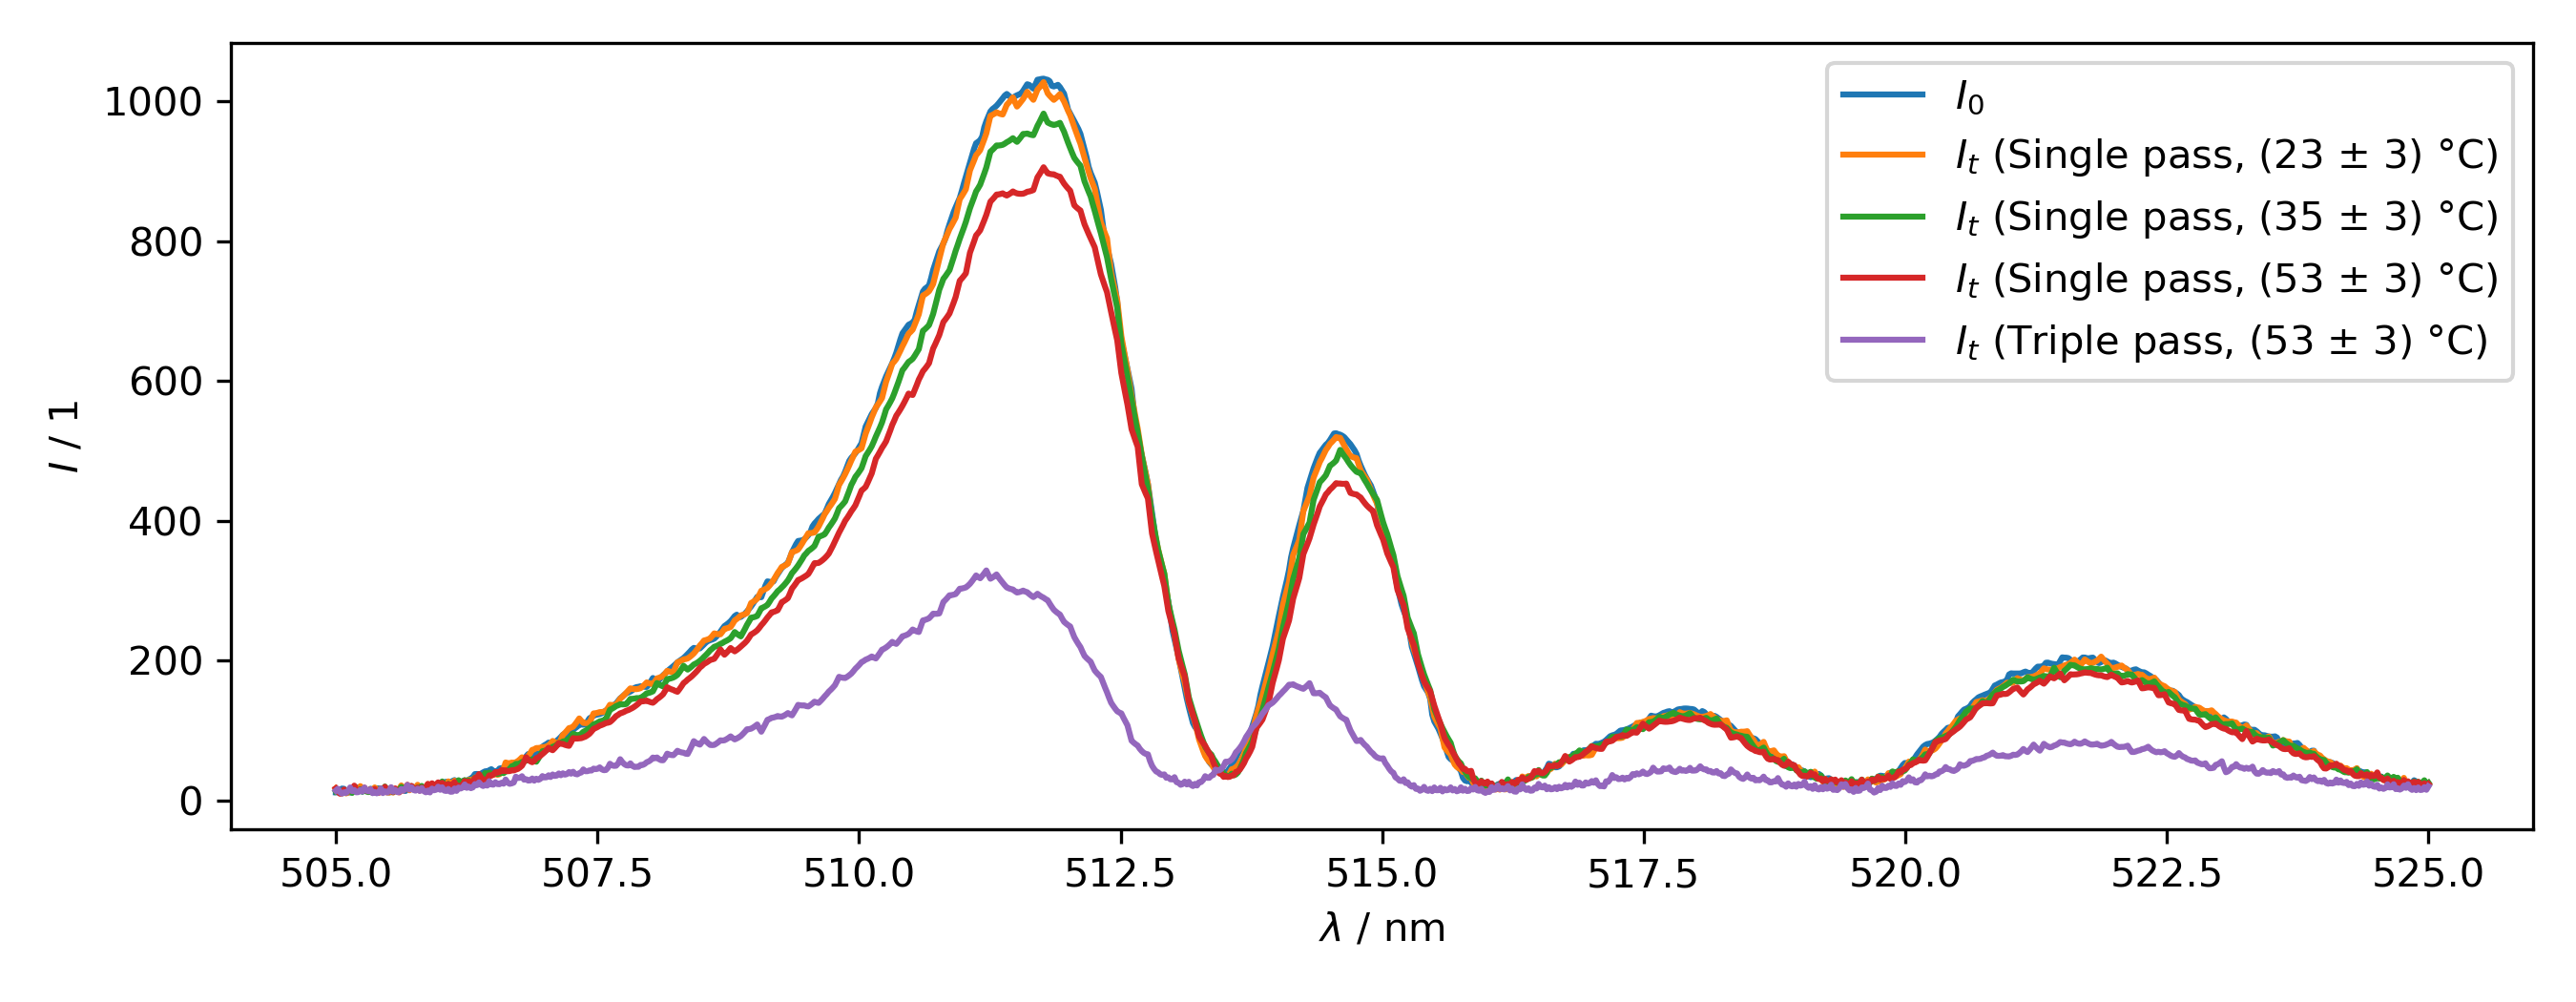
\includegraphics[width=\textwidth]{graphics/transmission.png}
    \caption{Transmission spectra without iodine as well as for single-pass and triple-pass configurations.\\
        $I_0$ = Intensity without iodine, $I_t$ = Intensity transmitted through iodine}
    \label{fig:evaluation:transmission}
\end{figure}

\begin{figure}[H]
    \centering
    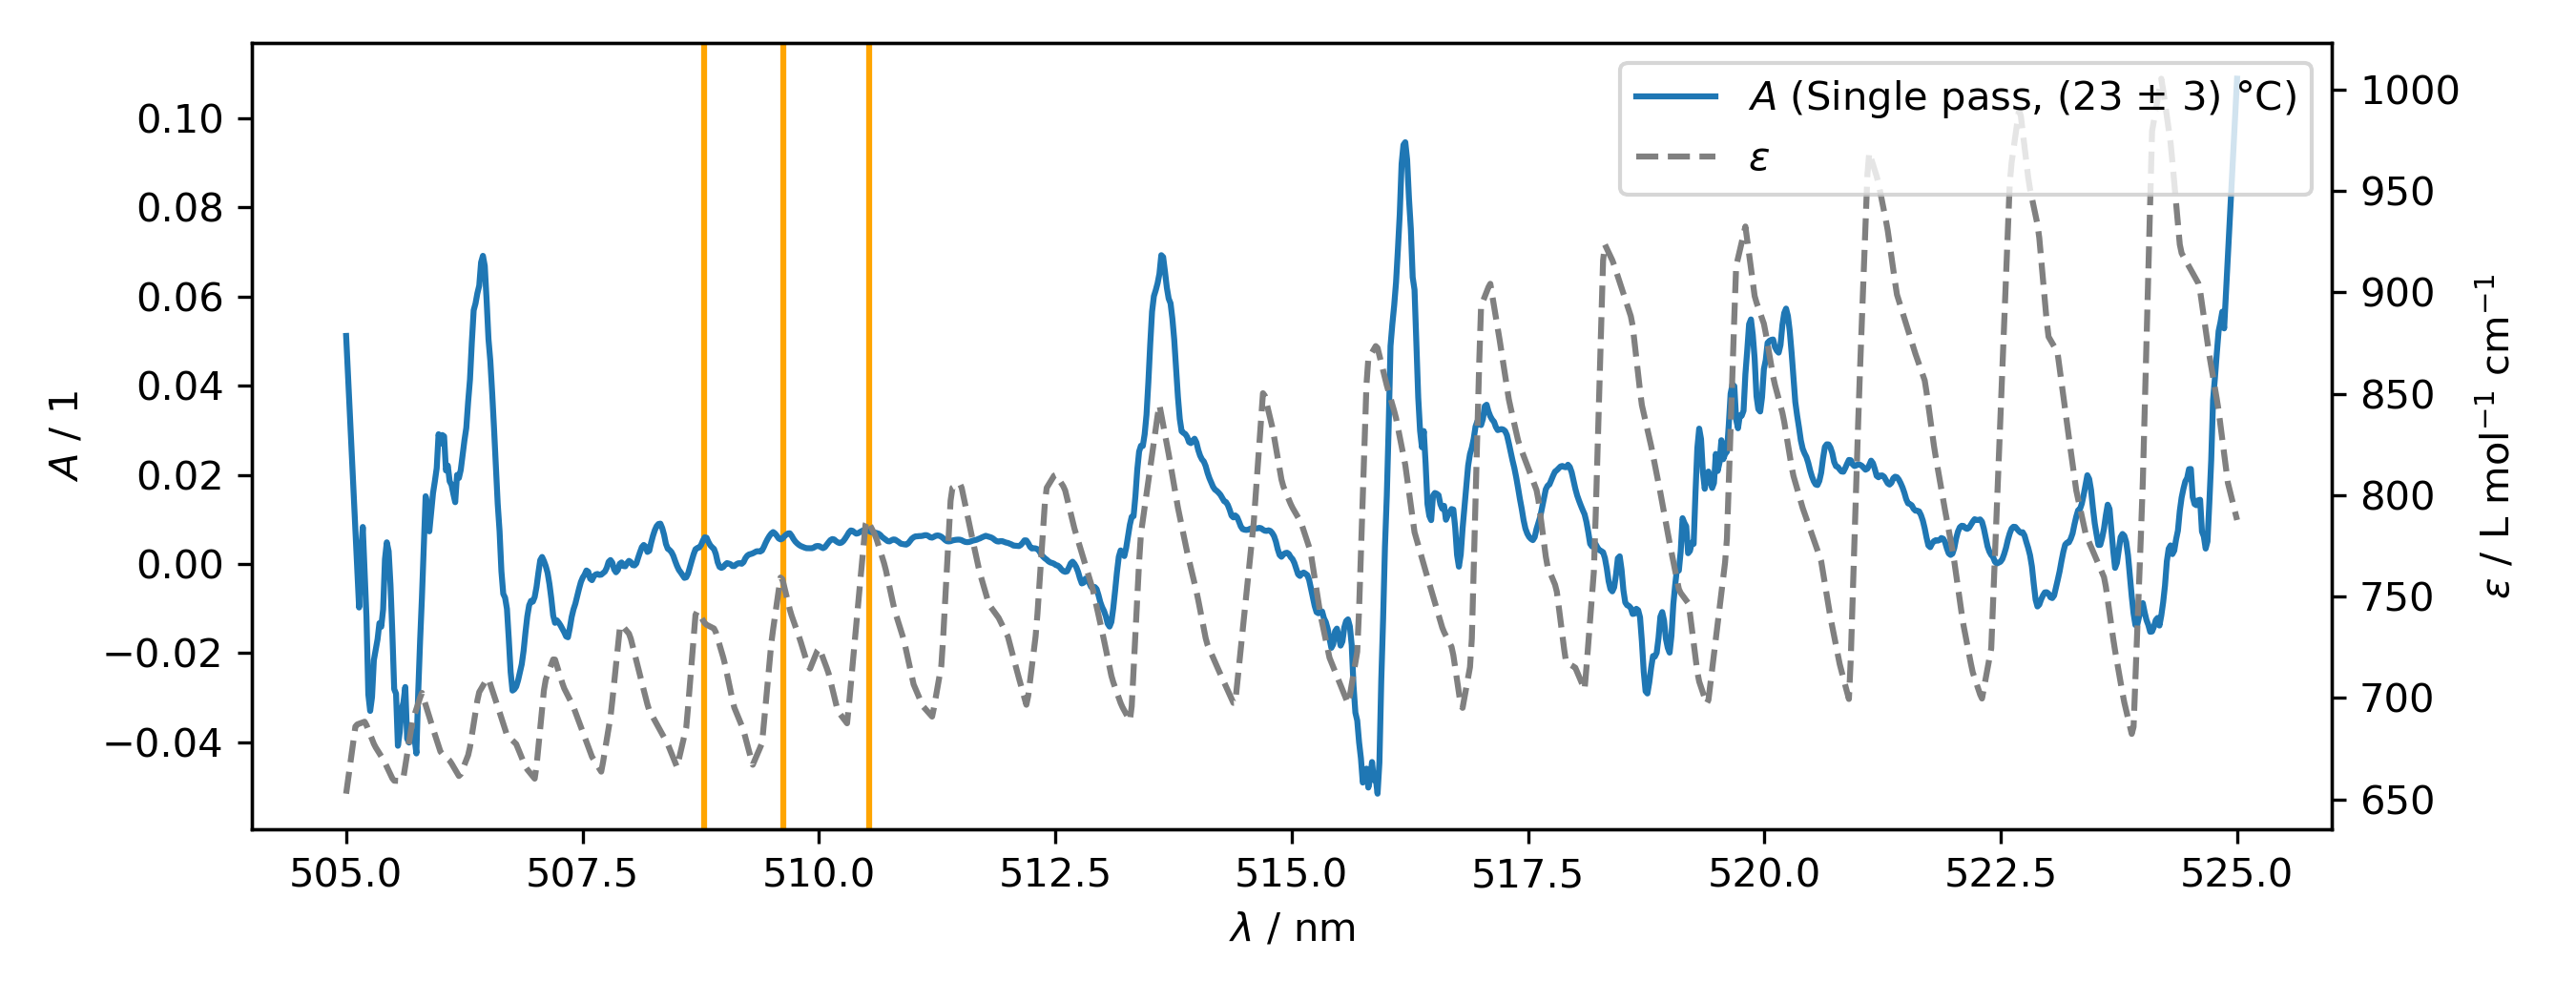
\includegraphics[width=\textwidth]{graphics/absorbance-25.png}
    \caption{Absorbance and used molar absorption coefficient as functions of wavelength.\\
        $A$ = Absorbance, $\varepsilon$ = Molar absorption coefficient, $\lambda$ = Wavelength}
    \label{fig:evaluation:absorbance:single:1}
\end{figure}

\begin{figure}[H]
    \centering
    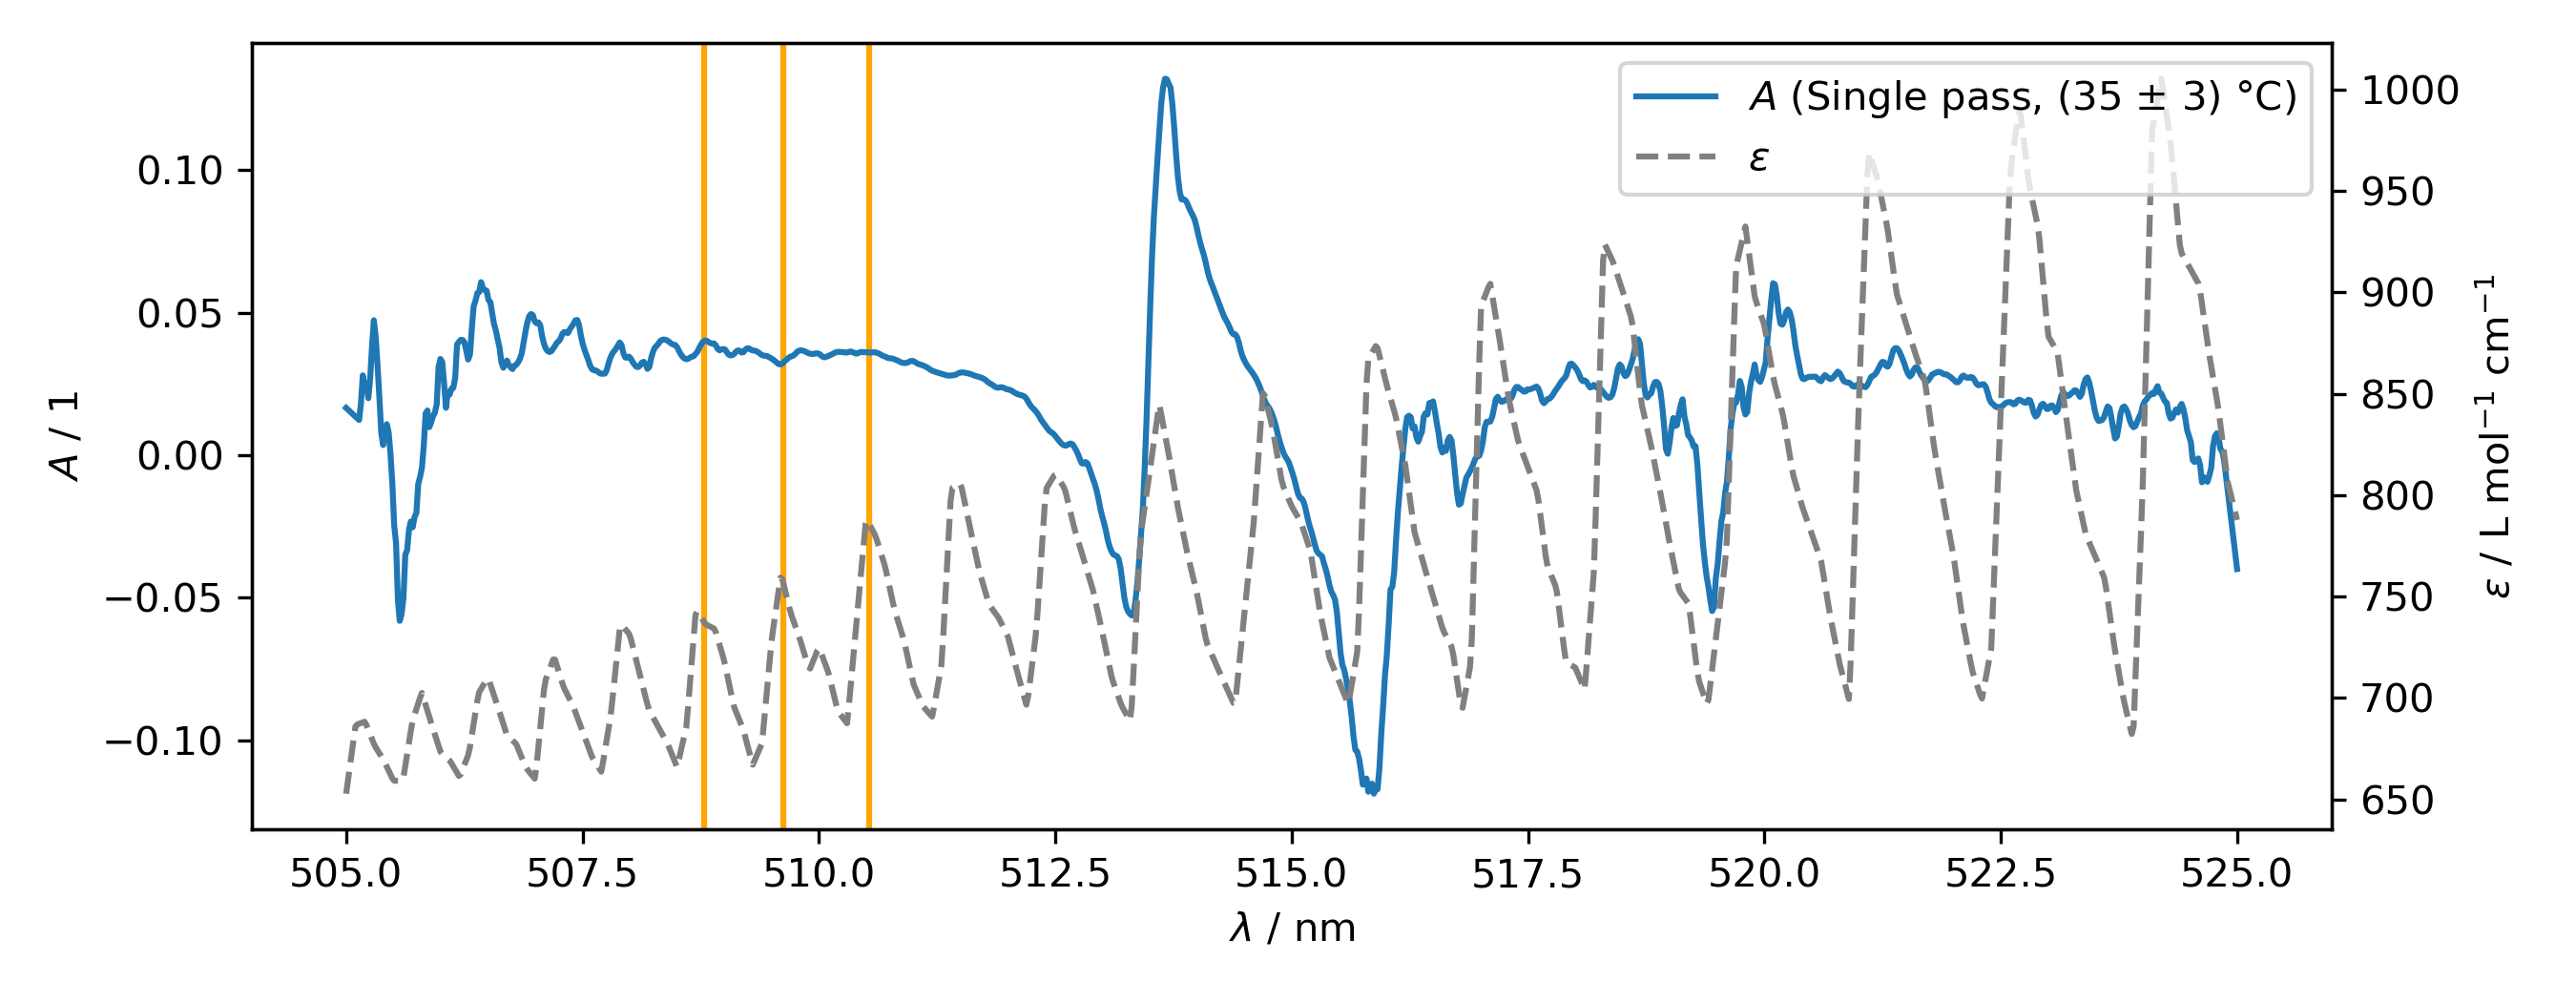
\includegraphics[width=\textwidth]{graphics/absorbance-42.png}
    \caption{Absorbance and used molar absorption coefficient as functions of wavelength.\\
        $A$ = Absorbance, $\varepsilon$ = Molar absorption coefficient, $\lambda$ = Wavelength}
    \label{fig:evaluation:absorbance:single:2}
\end{figure}

\begin{figure}[H]
    \centering
    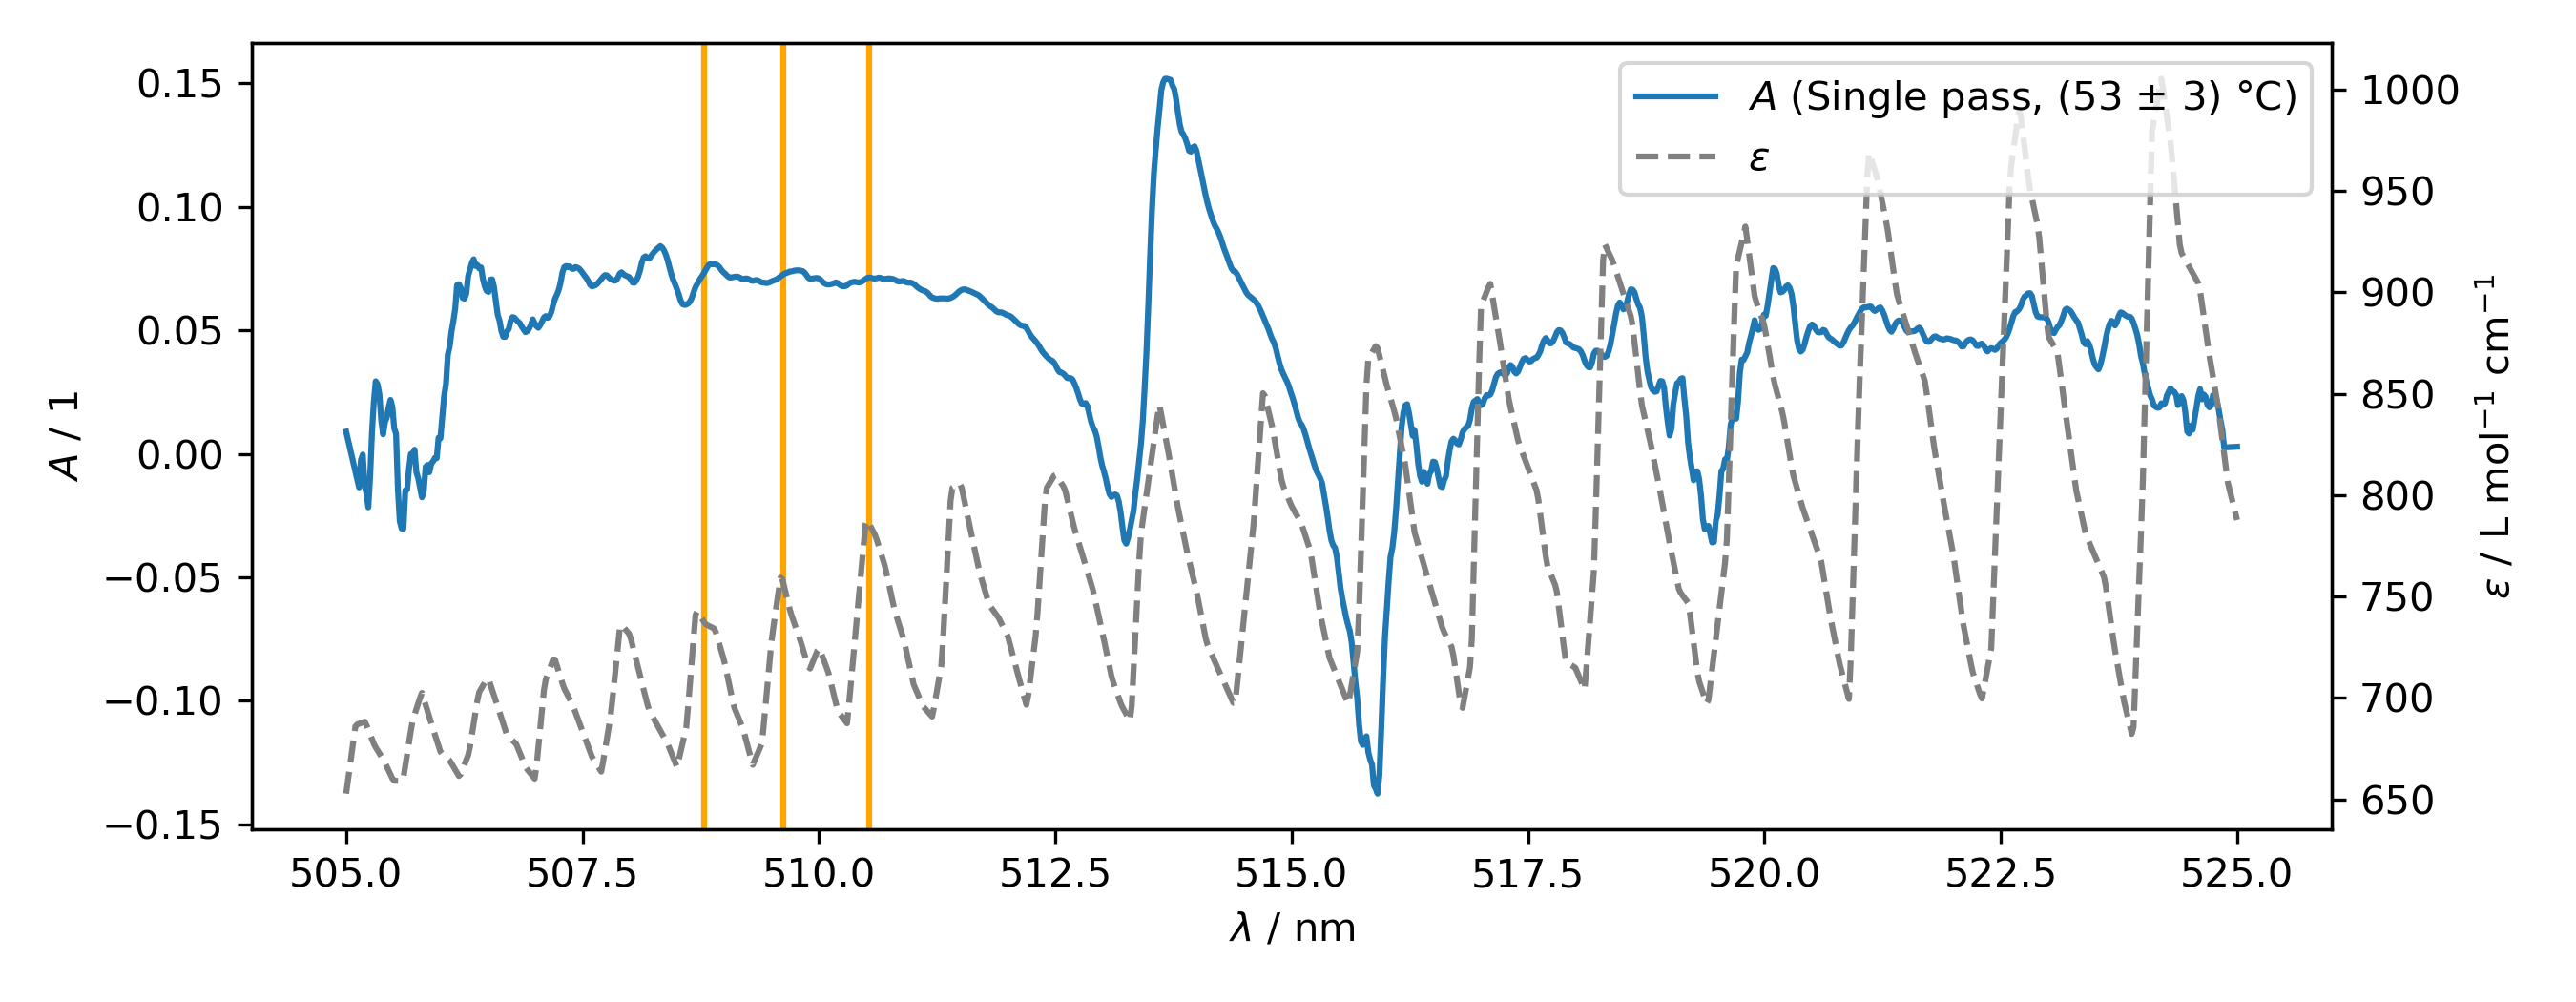
\includegraphics[width=\textwidth]{graphics/absorbance-60.png}
    \caption{Absorbance and used molar absorption coefficient as functions of wavelength.\\
        $A$ = Absorbance, $\varepsilon$ = Molar absorption coefficient, $\lambda$ = Wavelength}
    \label{fig:evaluation:absorbance:single:3}
\end{figure}

\begin{figure}[H]
    \centering
    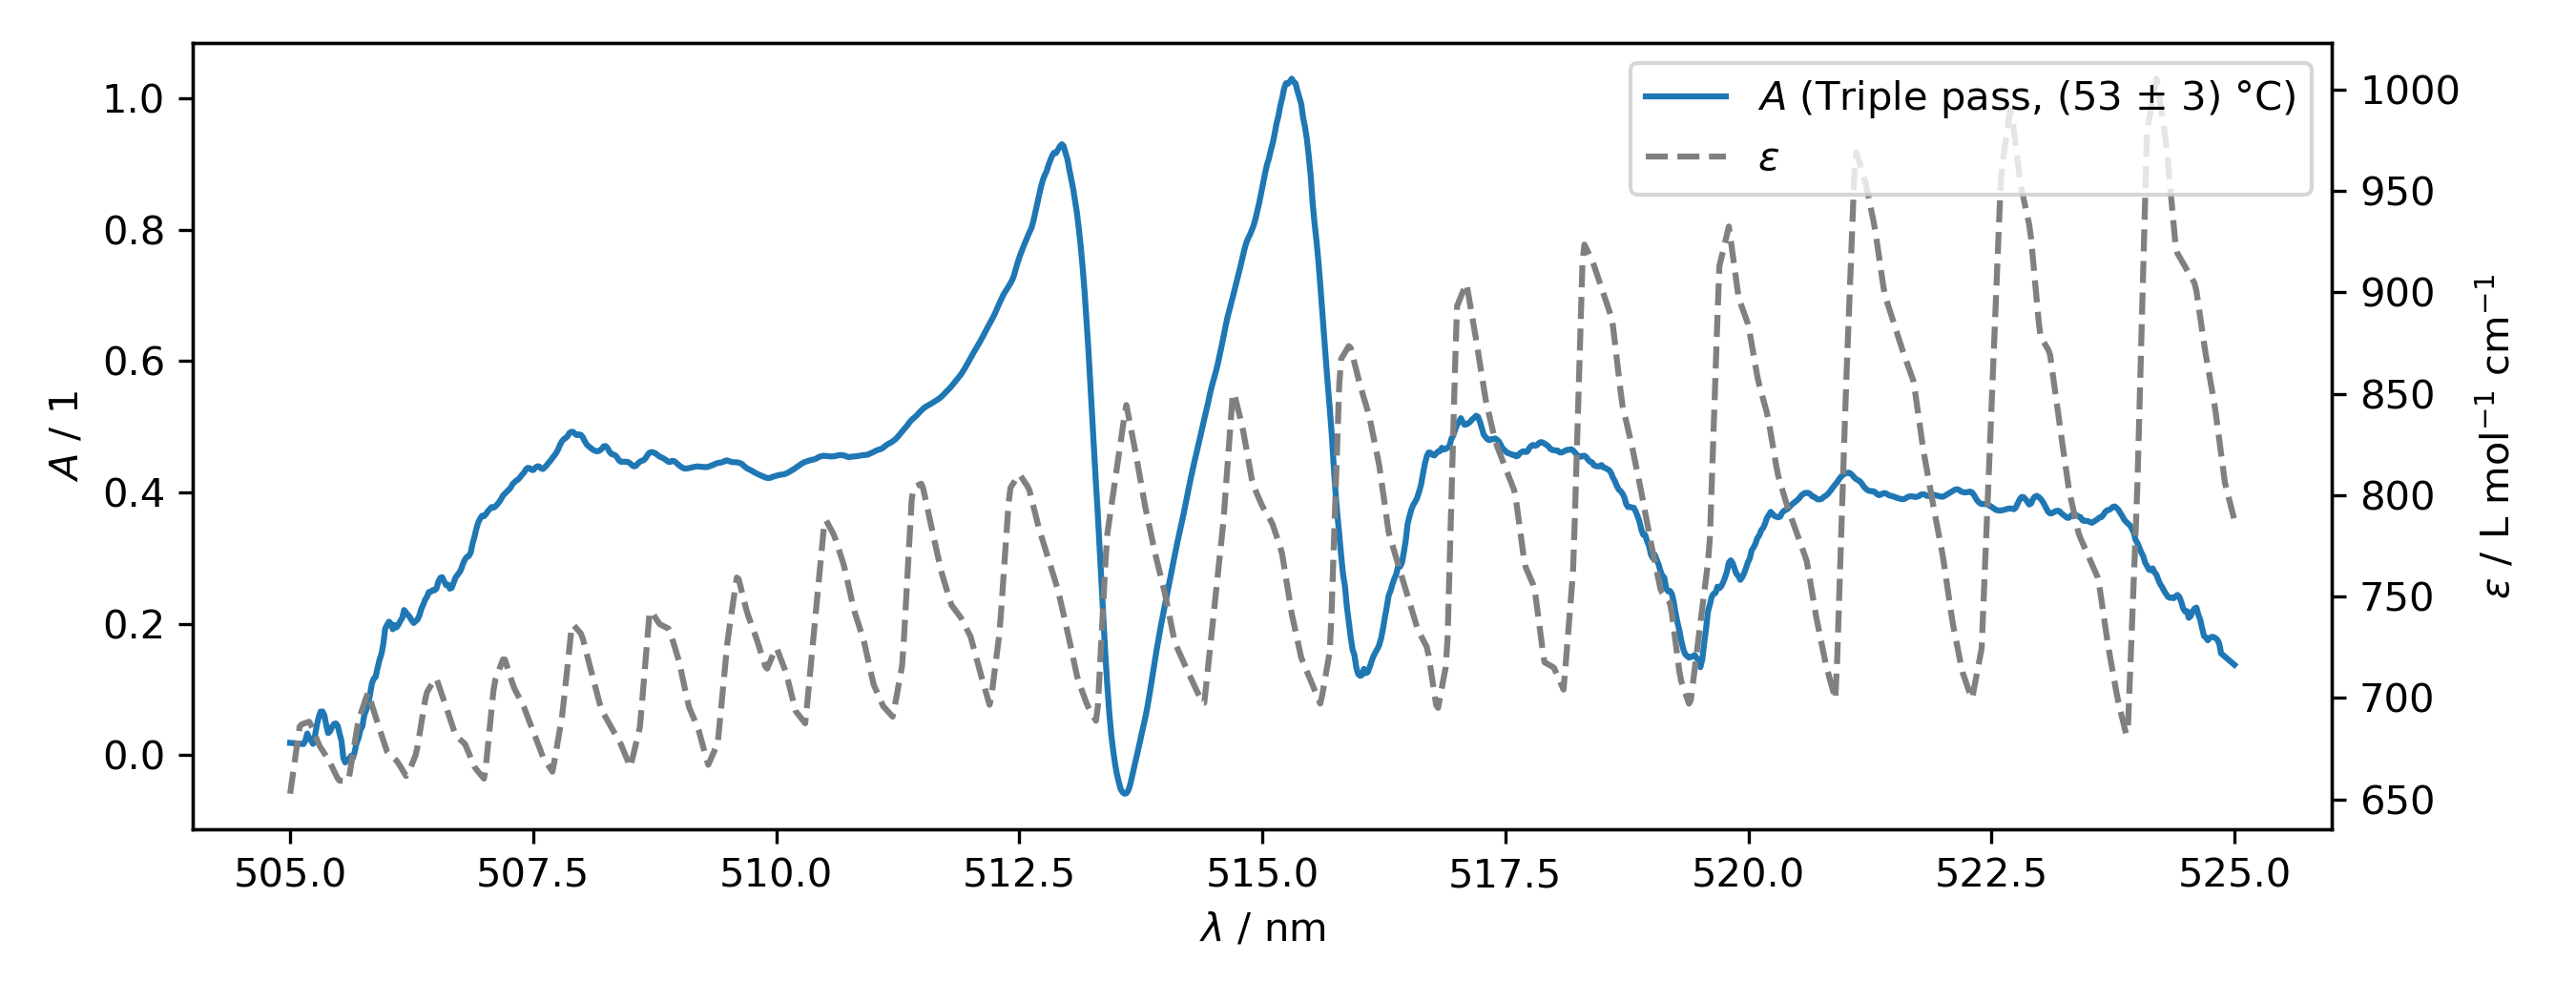
\includegraphics[width=\textwidth]{graphics/absorbance-triple.png}
    \caption{Absorbance and used molar absorption coefficient as functions of wavelength.\\
        $A$ = Absorbance, $\varepsilon$ = Molar absorption coefficient, $\lambda$ = Wavelength}
    \label{fig:evaluation:absorbance:triple}
\end{figure}

\subsection{Iodine Concentration}
\label{sec:evaluation:iodine-concentration}

Using Equation \ref{eq:fundamentals:beer} as well as the absorbance $A$ and molar absorption coefficient $\varepsilon$ obtained in Section \ref{sec:evaluation:iodine-absorbance}, the concentration $c$ of molecular iodine in the cell can be calculated.
For this, the effective path-length $l$ of the laser beam passing through gaseous iodine is required. Given the bases $l_l = \SI{98(2)}{\mm}$ and $l_s = \SI{90(2)}{\mm}$, the effective length of a single pass can be assumed to be $l = \SI{94(6)}{\mm}$, such that the uncertainty covers even extreme alignment conditions.

As further discussed in Section \ref{sec:discussion}, the spectra shown in the previous section suffer from various flaws, most prominent being the fact that negative absorbance $A$ due to intensity shifts created by changing the configuration of the setup is physically meaningless. For this reason it is safe to assume that the uncertainty of the spectrometer as documented in Table \ref{tab:equipment} is negligible compared to other uncertainties introduced due to imprecise experimental handling, for which a combined uncertainty $\Delta A = 0.2$ is used for further calculations. This uncertainty also includes intensity losses introduced due to mirrors, reflections as well as passes through the iodine cell glass walls.

Regarding the uncertainty of the molar absorption coefficient $\varepsilon$ it needs to be considered that the reference spectrum taken from literature \cite{Iodine} shows very distinctive absorption peaks compared to the absorbance $A$ acquired in the course of the present work. This leads to a combined uncertainty $\Delta \varepsilon = \SI{100}{\L\per\mol\per\cm}$ of approximately a peak height in the region of $\lambda = \SI{508}{\nm}$ to $\lambda = \SI{511}{\nm}$ being considered adequate.

Propagating the various uncertainties as discussed, Equation \ref{eq:fundamentals:beer} is used to calculate the concentration for all wavelengths in the range of $\lambda = \SI{508}{\nm}$ to $\lambda = \SI{511}{\nm}$. The final concentration is calculated as an arithmetic mean from this values, which yields the concentrations of iodine for various configurations as shown in Table \ref{tab:evaluation:concentration}. The plausibility of these values are further discussed in Section \ref{sec:discussion}.

\begin{table}[H]
    \centering
    \caption{Intensity spectrum for the infrared laser. \\
    $L \pm \Delta L$ = Effective total length, $T \pm \Delta T$ = Temperature, $c \pm \Delta c$ = Concentration}
    \label{tab:evaluation:concentration}
    \begin{tabular}{cccccc}
    \hline
    $L$ / mm & $\Delta L$ / mm & $T$ / \si{\celsius} & $\Delta T$ / \si{\celsius} & $c$ / \si{\m\mol\per\m^3} & $\Delta c$ / \si{\m\mol\per\m^3} \\ \hline
    94 & 6 & 23 & 3 & 1 & 2 \\
    94 & 6 & 35 & 3 & 5 & 2 \\
    94 & 6 & 53 & 3 & 11 & 3 \\
    192 & 18 & 53 & 3 & 22 & 3 \\ \hline
    \end{tabular}
\end{table}

\newpage
%************DISKUSSION***************
\section{Summary \& Discussion}
\label{sec:discussion}
\subsection{Laser Source Characterization}
As seen in the literature \cite{Koerner:12}, Ytterbium-doted gain medium indeed emit at wavelengths comparable with the acquired data.
It seems that the recorded intensity curve consists of at least seven emission lines with a bimodal tendency.
However, the possibility of overfitting is also plausible because the emission lines of a pulsed laser should be equidistant and dependent on the bandwidth of the medium and the length of the laser cavity.
With a FWHM of ($40.33 \pm 0.10$) nm, the bandwidth of the laser is relatively high.
This is expected for Ytterbium-based laser systems, as Ytterbium's high bandwidth enables it to build up several modes in the resonator cavity.
Therefore, it is favorable to use it for spectroscopic purposes, however this bimodal feature indicates that this laser is most likely not operating properly.


\subsection{SHG Characterization}
Unlike the fundamental spectrum of the laser, the SHG spectrum gives more clues to the nature of the laser.
The five peaks obtained show up in both spectra but are more prominent in the SHG spectra, which leads to the assumption that the laser has five modes.
It becomes also clear if looking at Figure \ref{fig:evaluation:shg_fitted} that some frequencies are more likely to be converted by the birefringent crystal.
It should also be noted that the conversion ratio obtained from the spectra is quite high, at over 80 \%.
This indicates good phase matching at the SHG crystal and an overall good alignment procedure.
However, as mentioned in \ref{sec:execution:shg-characterization}, the power measurement of the laser after the SHG stage shows that a lot of energy is lost in the system.
This could be due to the absorbtion and scattering of the photons over the optical axis, most likely in the SHG stage.
One problem with the calculated conversion rate is that its value is far too high because of the big loss of infrared light at the two mirrors after the SHG stage shown in Figure \ref{fig:setup:shg}.
These mirrors are designed for wavelengths at around 500 nm, which leads to a significant reduction of the residual spectrum.
One way around this fact is to use the fundamental spectrum without the SHG stage.
Only the intensity of the measured spectra in the grating spectrometer is vastly dependent on the level of optimization and, therefore, the alignment of the laser by adjusting the mirrors in the correct way.
There is no way to know if both spectra are taken at the maximum level of optimization.
More than that, it is quite likely that this is not the case because, as the optimization of the fundamental spectrum was made, it was possible to oversaturate the photodiode.
This means that the intensity exceeded the measurement range.
This was not possible to achieve with the SHG spectrum, indicating that the conversion rate must be far less than what can be calculated using the fundamental and SHG- spectra.
Therefore, the SHG- spectrum with the IR peaks was used under the assumption of energy conservation, which, as discussed before, cannot be valid.
For the sake of completion, the value was calculated using the other evaluation strategy:
\begin{equation}
    CR = (0.011 \pm 0.001) \hspace{2pt} \% \hspace{3cm} CR \ldots \text{Conversionrate}
\end{equation} 


\subsection{Iodine Absorbance}
\label{sec:discussion:iodine-absorbance}

Given the transmission spectra as shown in Figure \ref{fig:evaluation:transmission}, it quickly becomes obvious that modifications made to the setup configuration impact the relation of successively recorded spectra in a negative way. This is especially visible in the range of $\lambda = \SI{513}{\nm}$ to $\lambda = \SI{514}{\nm}$, where the transmitted intensity $I_t$ through the iodine cell in the triple-pass configuration at $T = \SI{53(3)}{\celsius}$ surpasses the initial intensity $I_0$ recorded without the iodine cell, which in an ideal setup without side-effects should not be possible.

This leads to the absorbance $A$ as shown in figures \ref{fig:evaluation:absorbance:single:1} to \ref{fig:evaluation:absorbance:triple} being negative for certain wavelengths $\lambda$, which of course is physically meaningless. As documented in Section \ref{sec:evaluation:iodine-concentration}, this leads to a relatively large uncertainty of $\Delta A = 0.2$ being chosen for further evaluation, which also accounts for intensity losses due to mirrors, reflections and passes through the glass walls of the iodine cell.

As further visualized in figures \ref{fig:evaluation:absorbance:single:1} to \ref{fig:evaluation:absorbance:triple}, the expected absorption peaks are hardly visible in most parts of the absorbance spectra for all configurations, being most prominent in the wavelength range of $\lambda = \SI{508}{\nm}$ to $\lambda = \SI{511}{\nm}$. It should be noted here that even these peaks are only visibly after applying a Savitzky–Golay filter with suitable parameters, while in the original spectrum it is hardly possible to distinguish the peaks from the surrounding noise.

While the position of the identified peaks match the positions shown in the spectra taken from literature \cite{Iodine}, the quality of the obtained absorbance spectra is far below expectations. In order to improve the results, potential issues of the setup used need to be considered.

One issue identified arises from the fact that using a laser as light source results in a rather narrow bandwidth of wavelengths $\lambda$, with wings of the line profile quickly approaching zero with increasing distance to the central wavelength. This makes detecting peaks even harder in addition to the high resolution that would already be required for uniformly distributed wavelengths $\lambda$ of the light source. Using either a laser directly capable of producing the required central wavelength without requiring a SHG stage or alternatively using some other sort of light source that produces coherent light of the required wavelength in a less concentrated wavelength interval is considered to be of advantage.

Another potential limiting factor that contributes to the noise of the obtained absorbance spectra stems from the fact that, as discussed in Section \ref{sec:fundamentals}, the used grating spectrometer does not offer unambiguous assignment of wavelengths $\lambda$ such as a prism spectrometer would provide. While for this reason using a prism spectrometer might be beneficial, the especially high reflectivity of the mirrors and gratings in the infrared region as well as the higher generally higher resolution still lead to the grating spectrometer being the device of choice.

While using a device with increased resolution is expected to improve results, the used grating spectrometer provides a resolution of up to \SI{0.05}{\nm}, which should be sufficient for properly resolving the absorption peaks as observed in the literature spectrum.

However, the main reason for the bad quality of the obtained spectra might be attributed to not closing the cover at the aperture of the spectrometer entrance slit, reducing spatial and spectral resolution due to large amounts of light entering the device, with ambient light additionally distorting measurements. While leaving the cover open can lead to an increased signal-to-noise ratio, this should not be a priority with the light source used. In subsequent experiments, it is therefore suggested to prefer resolution over signal-to-noise ratio and leave the cover at the input slit closed.

\subsection{Iodine Concentration}
\label{sec:discussion:iodine-concentration}

Considering the molar absorption coefficient $\varepsilon$ a shown in figures \ref{fig:evaluation:absorbance:single:1} to \ref{fig:evaluation:absorbance:triple}, which was calculated from the absorption cross-section $\sigma$, it becomes obvious that the values match with the values taken from further literature as shown in Figure \ref{fig:discussion:epsilon}.

This also applies to the calculated concentrations $c(T = \SI{23(3)}{\celsius}) = \SI{1(2)}{\milli\mol\per\m^3}$, $c(T = \SI{35(3)}{\celsius}) = \SI{5(2)}{\milli\mol\per\m^3}$ and $c(T = \SI{53(3)}{\celsius}) = \SI{11(3)}{\milli\mol\per\m^3}$ for the single-pass configuration as documented in Table \ref{tab:evaluation:concentration}. For example, as visualized in Figure \ref{fig:discussion:concentration}, for $T \approx \SI{35}{\celsius}$ at an absorbance of $A \approx 0.04$ the concentration is expected to be $c \approx \SI{0.6e-5}{\mol\per\liter} = \SI{6}{\milli\mol\per\m^3}$, which matches the obtained concentration of $c(T = \SI{35(3)}{\celsius}) = \SI{5(2)}{\milli\mol\per\m^3}$.

\begin{figure}[H]
    \centering
    \begin{minipage}[b]{0.49\textwidth}
        \centering
        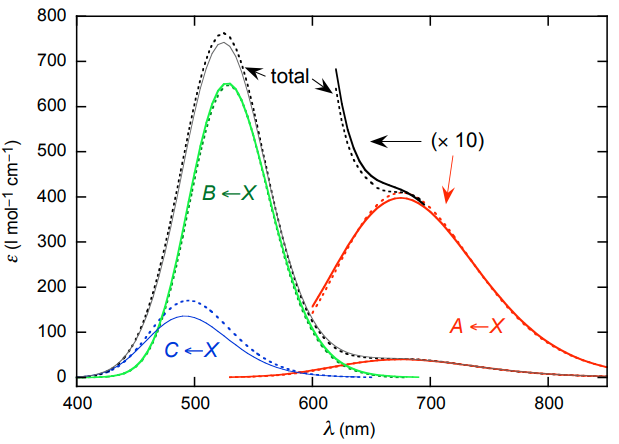
\includegraphics[width=0.9\textwidth]{graphics/literature-epsilon.png}
        \caption{Molar absorption coefficient $\varepsilon(\lambda)$ for molecular iodine at $T \approx \SI{35}{\celsius}$ \cite{tellinghuisen2011least}.}
        \label{fig:discussion:epsilon}
    \end{minipage}
    \hfill
     \begin{minipage}[b]{0.44\textwidth}
        \centering
        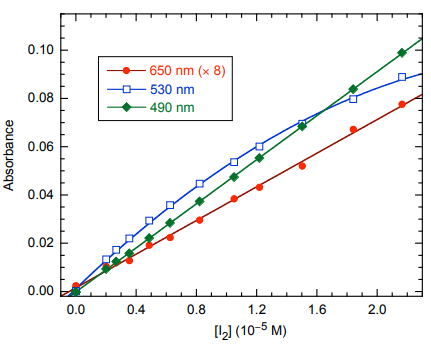
\includegraphics[width=0.9\textwidth]{graphics/literature-concentration.png}
        \caption{Absorbance $A(c)$ for molecular iodine at $T \approx \SI{35}{\celsius}$ \cite{tellinghuisen2011least}.}
        \label{fig:discussion:concentration}
    \end{minipage}
\end{figure}

The obtained concentrations $c$ for the single-pass configuration are therefore, at least with respect to orders of magnitude, assumed to be correct. However, for the triple-pass configuration at $T = \SI{53(3)}{\celsius}$, the obtained concentration amounts to $c = \SI{22(3)}{\milli\mol\per\m^3}$ as opposed to the corresponding single-pass value $c = \SI{11(3)}{\milli\mol\per\m^3}$.

This might - in addition to the reasons already mentioned in Section \ref{sec:discussion:iodine-absorbance} - be attributed to additional losses of intensity due to reflections and the increased number of cell wall passes the laser beam has to overcome in the triple-pass configuration.

To overcome this problem, it is advisable to not artificially extend the effective path-length of the laser beam in the iodine gas by use of mirrors, but to actually use dedicated iodine cells of matching length. Furthermore, it should be ensured the glass walls of the iodine cell only exhibit negligible interaction with the wavelengths of interest in order to not distort the measured transmitted intensity $I_t$. Alternatively, the absorbance of the glass walls could be determined in a separate experiment and then be compensated for in the evaluation. Also, the number of mirrors should not be changed between measurements to keep the intensity loss at the mirrors constant among different configurations.




%%************ZUSAMMENFASSUNG************
\section{Zusammenfassung}
\label{sec:zusammenfassung}
 

\section{Literature}
\printbibliography
\end{document}